\chapter{Task description}The overall task is to investigate and develop a service that allows to measure the latency an interrupt generates. This has to be achieved without external hardware and as accurate as possible with an AT91RD9200-EK development board. The service should be generic and independent in terms of the main functionality. One other point is, that the service ought to create less overhead and not extent the measured interrupt more than necessary. Further more the the measured value has to be converted into a time unit (e.g. $\mu s$) and be compensated to represent the real period the interrupt needed without the may influencing measure service. For the system output the values hast to be transmitted by any terms of connection to a host computer, running a database and stores the received values. For better readability it is recommended that the transmitted values are plain text. This allows easier debugging and also a stand alone operation without the running database. To trace back the recorded latencies timestamps should be provided to identify when and maybe under what conditions, excess length in interrupt routine occurred.\\


\chapter{Environment}
This chapter is a short introduction into the microcontroller and environment and software to program the chip. It provides information about the basic setup to get started with the controller plus the required software with the corresponding settings.\\

\section{The chip ATMEL AT91RM9200}
\label{atcore}
The chip AT91RM9200 is an ARM9-based microcontroller. The on \ac{RISC} based architecture features more than 1\ac{MIPS} per MHz. Several other features like low power consumption and two switchable instruction set are also present. Furthermore the chip hosts an \ac{AIC} which allows the system designer or programmer, a flexible and prioritized interrupt configuration. The 8-level priority allows nested interrupts. In general the processor has 16 registers. Table \ref{tab:regs} illustrates the register names and their functionality.

\begin{table}[H]
\begin{tabular}{lll} %\hline
\textbf{Register}	 &\textbf{Description} &\textbf{Notes}  \\
\hline
\hline
R0-R7 			& general-purpose Register & Registers are unbanked\\
R8-R12 			& general-purpose Register & Registers are banked in case of the \acs{FIQ}\\
R13 				& Stack pointer (software convention) & Banked register\\
R14 				& return address in an subroutine call & Banked register\\
R15					& \ac{PC} & Banked register\\
\hline
\hline
\acs{CPSR}	& \multicolumn{2}{l}{\acf{CPSR} containing:} \\
	& \multicolumn{2}{l}{$\bullet$ ALU flags (Negative, Zero, Carry, and Overflow)}\\
	& \multicolumn{2}{l}{$\bullet$ Interrupt disable bits}\\
  & \multicolumn{2}{l}{$\bullet$ One bit that indicates whether ARM or Thumb execution is used}\\
	&  \multicolumn{2}{l}{$\bullet$ The current processor mode (\textit{usr,fiq,irq,svc,abt,und,sys} see table \ref{tab:cpuMode})}\\


%\cline{1-2}

\end{tabular}
\caption{AT91RM9200 Registers}
\label{tab:regs}
\end{table}
The banked registers are in hardware separate registers accessed with the same hardware address. This means, that each register depends on the current processor mode. For the \ac{FIQ} there are more such banked registers. This allows a faster context switch with no need to save this registers. The \ac{FIQ}-\ac{ISR} should use the registers R8-R12 for the calculation or to process data. The interrupt entry and exit therefor could reduce the interrupt processor cycle count.\\
The chip also includes also a power management as well as a powerful debugging unit. Besides this there are several communication ports such as \ac{UART}, \ac{USB} or Ethernet located on the development board and supported by the core hardware.\\ 
Table \ref{tab:cpuMode} gives an overview about the different processor modes. Each mode has different privileges and priorities. The \ac{FIQ} for example can't be interrupted by the "normal" \ac{IRQ} and serves a fast response and low latency. To transmit data it can use the \ac{DMA} to send data with low \ac{CPU} load. In general most of the applications will run in the user mode. The other modes are used to access protected resources or serve exception handling.\cite{AT91Overview}\cite{AT91RTC}\cite{UNISTG}\\




\begin{table}[H]
\begin{tabular}{lll} %\hline
\textbf{Processor Mode} &\textbf{Mnemonic}	 &\textbf{Description / Usage}  \\
\hline
\hline
  User&\textit{usr}& Standard (user) execution state\\
  FIQ&\textit{fiq}& Fast data / interrupt processing mode\\
  IRQ&\textit{irq}& Used for General-purpose interrupts\\
  Supervisor&\textit{svc}& Protected mode for the operating system\\
  Abort mode&\textit{abt}& Implements virtual memory and/or memory protection\\
  System&\textit{sys}& Privileged mode for the operating system\\
  Undefined&\textit{und}& Mode for undefined instructions\\

\end{tabular}
\caption[Processor Mode]{Processor Mode \cite{AT91Overview}\cite{AT91RTC}\cite{UNISTG}}
\label{tab:cpuMode}
\end{table}








\section{WinARM}
The WinARM-package is collection of GNU and other ARM developing tools. It is supposed to run on Windows as host computer and includes with the GCC (compiler,linker and assembler) the way to generate target code. This one is needed, because the host system (in this project Windows 7) differs from the ARM-architecture and so the GCC takes over the part, as a cross compiler, of creating this ARM-specific target code.\\
To get started with the WinARM package download an actual version (used one: \href{http://www.siwawi.arubi.uni-kl.de/avr_projects/arm_projects/WinARM-20060606.exe}{WinARM-20060606}) of the package, extract and install it. For best practice locate the files in system root (C:\textbackslash WinARM).\\
Then the following lines needs to be added to the system variable "Path":
\begin{itemize}
	\item C:\textbackslash WinARM\textbackslash utils\textbackslash bin;
	\item C:\textbackslash WinARM\textbackslash arm-elf\textbackslash bin;
	\item C:\textbackslash WinARM\textbackslash bin;
\end{itemize}

\section{Programmers Notepad 2}
To be able to compile a program the \ac{PN2} need to be \textbf{run as Administrator}, otherwise the software does not have the right privileges to pass parameters to the compiler. Therefor right click on the \ac{PN2}.exe and select "Run as administrator". For the actual build the make-file hast to be opened inside the \ac{PN2} and then select "Tools" from the menu bar and click "Make all". This will generate all, by the make-file specified, files. The actual file-name for the output files is declared inside the "config.mk"-file as TARGET (in this project: {\textcolor{black}{TARGET}}= project\_win).\\

\section{TFTP-Server} 
The \ac{TFTP} is a file transfer protocol and is used in the project to transfer the core configuration file to the BDI2000. One characteristic compared to a FTP-Server is, that the \ac{UDP} based \ac{TFTP} does not provide mechanism for authentication.\cite{TFTPWIKI}\\
The \ac{TFTP}-Server is also used to transfer the compiled runnable to the Microcontroller. Therefor the \ac{TFTP}-Server should contain the flash and also the configuration file.\\

\subsection{BDI-Configuration-File}
Besides the initialization of flash, clocks and \ac{RAM}, the configuration file contains information about the target e.g. the \ac{CPU}-type.\\
The [HOST]-section (Listening \ref{CFGFile}) comprises the Host-IP. The \ac{TFTP}-Server has to use this IP-address to enable the BDI to connect and load the configuration file. The FILE parameter provides the default file name which loaded via the Telnet (see section \ref{TEL}) if no other file name is specified. The PROMPT can be also customized and is a good way to check if the configuration is loaded correctly. The START option is the address where the \ac{CPU} starts if no other address is specified in the run command.\\
\begin{lstlisting}[language=C, caption={Extract of the rm9200dk.cfg-file}, label={CFGFile}]
[HOST]

IP          10.0.0.100
FILE	    	project_win.bin	
FORMAT	    BIN 0x20000000
LOAD        MANUAL      		;<AGENT> load VxWorks code MANUAL
PROMPT      Chris@BDI>      ;new Telnet prompt
DEBUGPORT   2001
START	    	0x20000000
\end{lstlisting}



\section{Telnet} 
\label{TEL}
Telnet is a widely common protocol to connect clients to their servers. It works across different platforms like Windows, Unix or Mac OS. How ever the TCP-based connection is rather insecure, because all data is transmitted as plain text including passwords for example.\\
The protocol is separated into two parts. The server is located at the BDI2000. The notebook needs to connect to the server via a Telnet-client. For best practice use PuTTY to connect to the BDI. The configuration setting is IP:\textit{10.0.0.101}, Port: \textit{23} and \textit{Telnet} as connection type.\\
The most useful work and debug commands are listed in Table \ref{tab:BDIComands}.\\

\subsection{BDI2000 Telnet command's} 

After a successful make of the source code, the target binary is located with in the same directory where the \ac{TFTP}-server has access. There is no need for a user or password login. After the first power up the BDI requests the "rm9200dk.cfg"-file. Therefor the \ac{TFTP}-server has to be started and the configuration file need to be provided. Otherwise the BDI replies inside Telnet with "\# CONFIG: cannot open rm9200dk.cfg". The transfer of this file could be seen inside the \ac{TFTP}-window. A second file, the "reg9200.def" is also transmitted, and is used to access hardware addresses by their mnemonics. If all cables are connected correctly (see system overview \ref{sysoverview} for details) the target messages a successful startup.\\
To get started and run the target binary, these three simple commands has to be entered in the terminal:
\begin{enumerate}
%\setlength{\itemsep}{2pt}
	\item \textbf{\textit{halt}} // Forces target into debug mode. Displays also the Contend of \ac{PC} and \ac{CPSR}
	\item \textbf{\textit{load}} // Loads the (default) program	to the target memory
	\item \textbf{\textit{go  }} // Sets the (default) \ac{PC}-address and starts the target 
	\end{enumerate}

The reg9200.def-file hosts information about the address and size in memory. Therefor the "RD"-command can be used with the the corresponding mnemonic. For all not described register addresses the more general "MD"-command has to be used. For example the value of a variable could be debugged with the "RD/RM"-command (variable address is known in the "project\_win.map"-file)
The following table \ref{tab:CCM} gives an example of two possible ways of reading and modifying commands for the \acs{RTC}-register.
\begin{table}[H]
\begin{tabular}{lll} %\hline
\textbf{Command}	 &\textbf{Access}&\textbf{Description}\\
\hline
\hline
RD RTC\_TIMR & Read& Reads the \acs{RTC}-time register\\% (hosting: meridiem indicator, hour, minute and second in \acs{BCD}-format\\
MD 0xFFFFFE08 1& Read& Same as RD RTC\_TIMR, 1 $\hat{=}$ 32bit word\\
\hline
RM RTC\_TIMR 0x00134530& Write& Sets the time to 13:45:30 \\%in the \acs{RTC}-time register\\
MM 0xFFFFFE08 0x00134530& Write& Same as RM RTC\_TIMR 0x00134530\\
\end{tabular}
\caption[Example of r/w access of the \acs{RTC} time register]{Example of r/w access of the \acs{RTC} time register\footnotemark}
\label{tab:CCM}
\end{table}
\footnotetext{To set a time, the \acs{RTC}-control register needs to be modified first (see \ref{RTCchapter} for details)
}



\begin{table}[H]
\begin{tabular}{ll} %\hline
\textbf{Command}	 &\textbf{Description}\\
\hline
\hline
MD [<address>] [<count>] & display target memory as word (32bit)\\
%MDH [<address>] [<count>] & display target memory as half word (16bit)\\
%MDB [<address>] [<count>] & display target memory as byte (8bit)\\
%DUMP <addr> <size> [<file>] & dump target memory to a file\\
MM <addr> <value> [<cnt>] & modify word(s) (32bit) in target memory\\
%MMH <addr> <value> [<cnt>] & modify half word(s) (16bit) in target memory\\
%MMB <addr> <value> [<cnt>] & modify byte(s) (8bit) in target memory\\
%MT <addr> <count> &memory test\\
%MC [<address>] [<count>] & calculates a checksum over a memory range\\
%MV &verifies the last calculated checksum\\
RD [<name>] & display CPU or user defined register\\
%RDFP &display floating point registers\\
%RDUMP [<file>] & dump all user defined register to a file\\
RM <name> <value> &modify CPU or user defined register\\
%TLB <from> [<to>] & display TLB entry (only V4e cores)\\
%WTLB <idx> <epn> <rpn> &write TLB entry (only V4e cores)\\
RESET &reset the target system\\
BREAK [SOFT | HARD] & display or set current breakpoint mode\\
GO [<pc>] & set PC and start target system\\
TI [<pc>] & single step an instruction\\
HALT &force target to enter debug mode\\
BI <addr> &set instruction hardware breakpoint\\
CI [<id>] & clear instruction hardware breakpoint(s)\\
%BD [R|W] <addr> &set data watchpoint (32bit access)\\
%BDH [R|W] <addr> &set data watchpoint (16bit access)\\
%BDB [R|W] <addr> &set data watchpoint ( 8bit access)\\
%CD [<id>] &clear data breakpoint(s)\\
INFO &display information about the current state\\
LOAD [<offset>]  [<file> [<format>]] & load program file to target memory\\
%VERIFY [<offset>]  [<file> [<format>]] & verify a program file to target memory\\
%ERASE <addr> <step> <count> &erase multiple flash sectors\\
%UNLOCK [<addr> [<delay>]] & unlock a flash sector\\
%UNLOCK <addr> <step> <count> &unlock multiple flash sectors\\
%DELAY <ms> &delay for a number of milliseconds\\
%HOST <ip> &change IP address of program file host\\
%PROMPT <string> &defines a new prompt string\\
CONFIG &display or update BDI configuration\\
HELP &display command list\\
%BOOT [loader] & reboot the BDI and reload the configuration\\
QUIT &terminate the Telnet session\\

\end{tabular}
\caption[Extract BDI2000 command list]{Extract BDI2000 command list\cite{BDIUSERMAN}}
\label{tab:BDIComands}
\end{table}

\section{System overview}
\label{sysoverview}
Figure \ref{fig:sysov} visualize an overview of the system. The figure only indicates the data connection. Each device is powered individual via battery or cable.\\
The host running the \ac{TFTP} and Telnet-servers is connected via Ethernet to the BDI2000. The IPs have to be assigned in a static way. The computer uses Telnet and the corresponding commands, specified in the \autoref{TEL}, to connect to the BDI2000. The BDI itself connects to the AT91RM9200 via a \ac{JTAG}-interface. The Development board with all its interfaces is connected to a computer via a bidirectional \ac{UART}. The interface itself and its settings, are described in \autoref{sec:RS232}. The user RS232 connection is used in this project to transmit the measurement values in a formatted way. The demo interrupt input is connected via a \ac{DIO} of the development board. The board also provides the power for the infrared based distance sensor, through the \ac{USB} 5V power supply. This ensures also a common ground, need to read the input voltages correctly.\\ 
In the case of programming the data flow is only between the computer and the BDI, as well as between the BDI and the development board.\\
For the demo application and the \ac{ILMS} (descried in \autoref{sec:ILMS}) the data flow is the following. The input sensor detects an obstacle in range. The output of the sensor turns to high level. The microcontroller process this interrupt. The \ac{ILMS} is started and as soon as there is no object, in reach of the sensor, stopped again. The result then is transmitted via the user serial communication to an computer running the database software. This could be the host computer, running the development environment or a separate one.

\begin{figure}[H]
		\begin{center}

	% Define block styles
    
\tikzstyle{block} = [rectangle, draw=blue, drop shadow,very thick,top color=white,              % a shading that is white at the top...
    bottom color=blue!20!,%fill=blue!20, 
    text width=8.5em, text centered, rounded corners, minimum height=5em,node distance=4cm,]
 
 \tikzstyle{blockred} =  [rectangle, draw=red, drop shadow,very thick,top color=white,              % a shading that is white at the top...
    bottom color=red!20!,%fill=blue!20, 
    text width=8em, text centered, rounded corners, minimum height=5em,node distance=3cm,]
\tikzstyle{blockgreen} = [rectangle, draw=green, drop shadow,very thick,top color=white,              % a shading that is white at the top...
    bottom color=green!20!,%fill=blue!20, 
    text width=8em, text centered, rounded corners, minimum height=5em,node distance=3cm,]

\tikzstyle{blocksmall} = [rectangle, draw=blue, drop shadow,very thick,top color=white,              % a shading that is white at the top...
    bottom color=blue!20!,%fill=blue!20, 
    text width=2em, text centered, rounded corners, minimum height=2em,node distance=3cm,]
 

\tikzstyle{line} = [draw,line width=1.0pt, -latex']
\tikzstyle{dblarrow} = [thick,<->,shorten >=1pt,shorten <=1pt,>=stealth, -latex']
\tikzstyle{line2} = [thick,->,shorten >=1pt,shorten <=1pt,>=stealth, -latex']
    
\begin{tikzpicture}[node distance = 2cm, auto]
    % Place nodes
\node [block] 		(pc) {Computer\\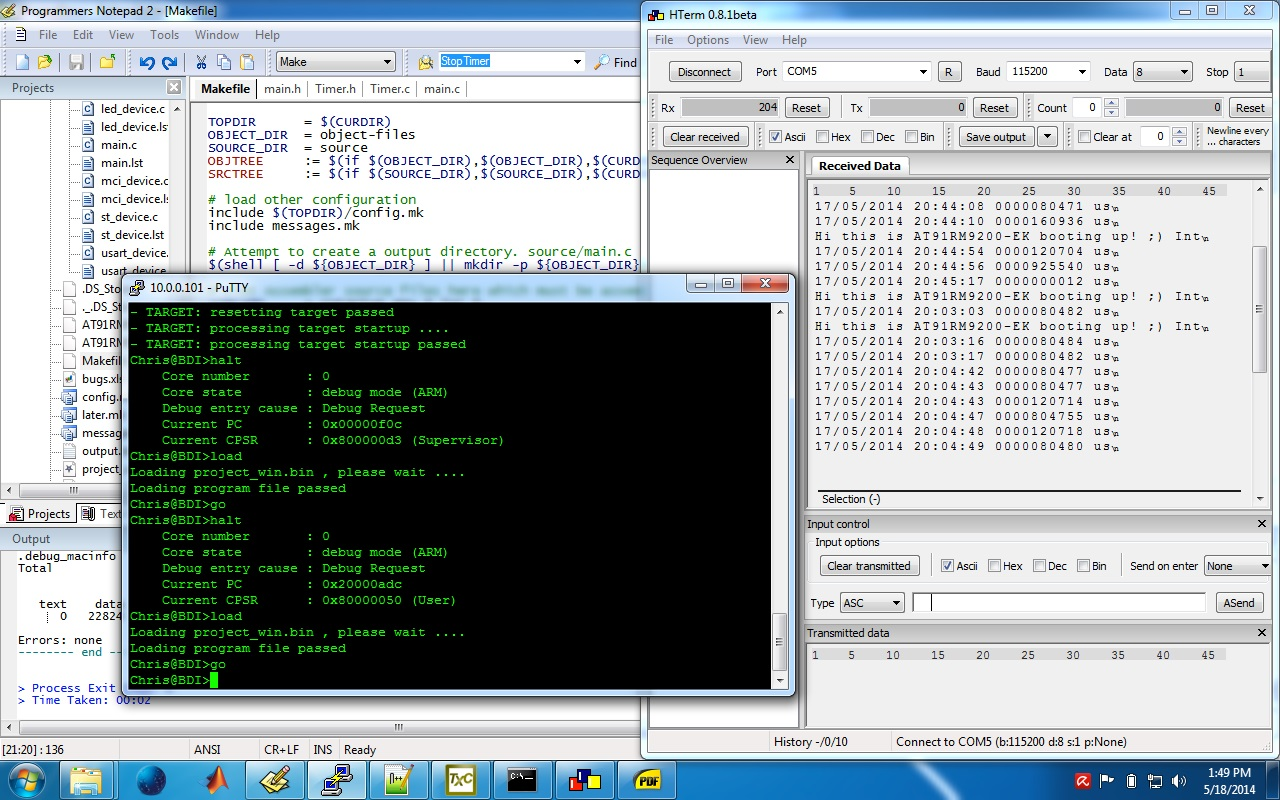
\includegraphics[height=4em]{images/IDE.jpg}};
\node [block, right of=pc, xshift=4cm] 		(BDI) {BDI2000\\ 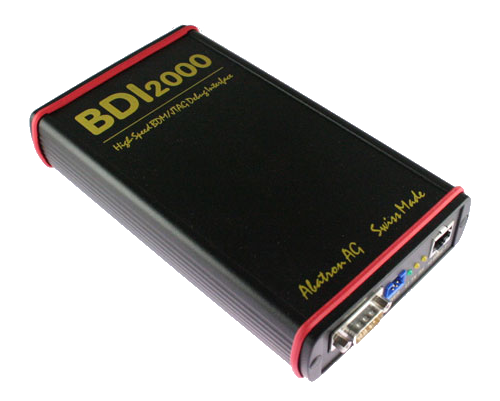
\includegraphics[height=4em]{images/bdi2000.png}};
\node [block, below of=pc] 		(IO) {Input Sensor\\ 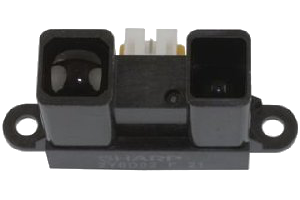
\includegraphics[height=4em]{images/GP2Y0D02YK0F.png}};
\node [block, below of=BDI] 		(AT) {AT91RM9200\\ 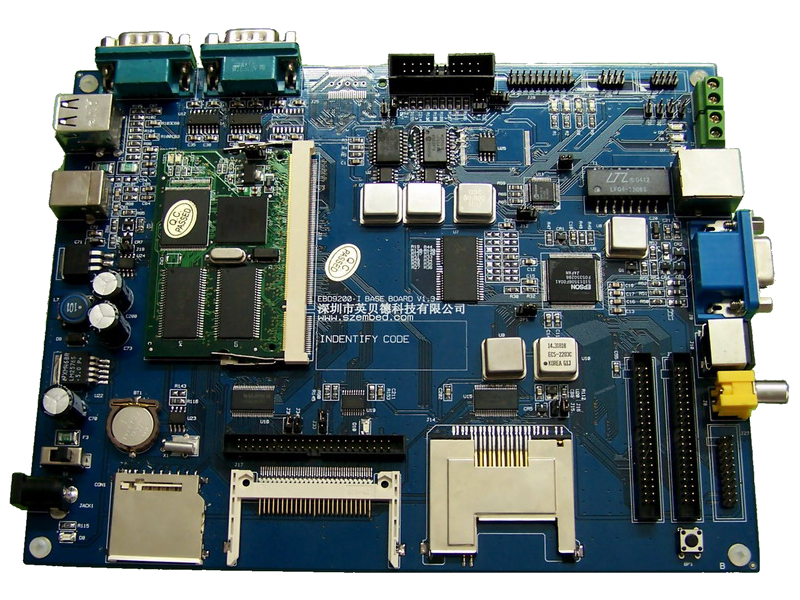
\includegraphics[height=4em]{images/AT91RM9200DB.png}};
%\node [block] 	(um2) {Umrechnung\\ SollTrq $\Rightarrow$ SollPos \\ };
%\node [block,  below of=abstmp] 	(tempmod) {$\Delta$-Temperatur- \\Algorithmus\\  };
%\node [blocksmall,  right of=tempmod, node distance=4cm] 	(multi) {$\times$};
%\node [blocksmall,  right of=multi, node distance=4cm] 	(multi2) {$\times$};
%\node [blocksmall,  above of=multi2] 	(divi) {$\div$};
%\node [blocksmall,  above of=divi] 	(minus) {$-$};
	%
 %
    %% Draw edges
    %\path [line] ([xshift=-2cm,yshift=+0.5cm] abstmp.west)--node [midway, above]{$Act_{Pwr}$}([yshift=+0.5cm] abstmp.west);
%\path [line] ([xshift=-2cm,yshift=-0.5cm] abstmp.west)--node [midway, above]{Tumg}([yshift=-0.5cm] abstmp.west);   
%
%
%\path [line] ([xshift=-2cm,yshift=+0.7cm] tempmod.west)--node [midway, above]{$P_{Eng\_Last}$}([yshift=+0.7cm] tempmod.west);
%\path [line] ([xshift=-2cm ] tempmod.west)--node [midway, above]{$nmot$}( tempmod.west);
%\path [line] ([xshift=-2cm,yshift=-0.7cm] tempmod.west)--node [midway, above]{vfzg}([yshift=-0.7cm] tempmod.west);   
%
%
\draw [dblarrow,<->] ([yshift=0.25cm]pc.east)--node [midway, above]{Ethernet, Telnet}([yshift=0.25cm]BDI.west);  
%\path [line] ([yshift=0.25cm]BDI.west)--node {}([yshift=0.25cm]pc.east);

\draw [dblarrow,<->] (BDI.south)--node [midway, right]{JTAG}(AT.north); 
%\path [line] (AT.north)--node {}(BDI.south); 

\draw [line2] ([yshift=-0.25cm]IO.east)--node [midway, below]{Digital Input}([yshift=-0.25cm]AT.west); 
\draw [dblarrow,<->] ([yshift=-0.25cm]pc.east)--([yshift=-0.25cm,xshift=2cm] pc.east)|-node [near start, above ,rotate=270]{\acs{UART}, RS232}([yshift=0.25cm] AT.west);
%\path [line] ([yshift=0.25cm]AT.west)-|([yshift=-0.25cm,xshift=2cm] pc.east)--([yshift=-0.25cm] pc.east);

%\path [line] ([xshift=-2cm] um2.west)--node [midway, above]{{SollTrq}}(um2.west); 
%\path [line] (abstmp.east)-|node [pos=0.27, above]{$Load_{Fact}$}( multi.north); 
%\path [line] (multi.east)--node [midway, above]{Gew. $\Delta T_{Hydr}$}( multi2.west);  
%\path [line] ([xshift=2cm] multi2.east)--node [midway, above]{$Vol_{Hyd1K}$}(multi2.east);
%\path [line] (multi2.north)--node [midway, above, rotate=90]{$\Delta Vol_{Hydr}$}(divi.south);
%\path [line] ([xshift=-2cm] divi.west)--node [midway, above]{{$Aktor_{Area}$}}(divi.west);   
%\path [line] (divi.north)--node [midway, above, rotate=90]{$Act_{Poscor}$}(minus.south);
%\path [line] (um2.east)--node [midway, above]{$SollPos$}(minus.west);
%\path [line] ( minus.east)--node [midway, above]{$SollPos_{Cor}$}([xshift=2cm] minus.east);
\end{tikzpicture}

		\end{center}
		\caption{System Overview}
		\label{fig:sysov}
\end{figure}


\chapter{Hardware abstraction}
In order to achieve an independent application a \ac{HAL} is introduced in the project. The basic idea is to have a strong decoupling between the different layers in the project. \autoref{fig:Layout} displays the implemented structure. The benefit of this layout is, that with the same \ac{HAL} and therefor the same \ac{API}, a switch to an other target hardware could be realized with no or little changes to the already running application. The so generic designed functionality allows scalability, extendability and hardware independence. Debugging or even the simulation of the application on the host computer is possible.\\
\begin{figure}[H]
		\begin{center}
			% Define block styles
    
\tikzstyle{block} = [rectangle, draw=blue, drop shadow,very thick,top color=white,              % a shading that is white at the top...
    bottom color=blue!20!,%fill=blue!20, 
    text centered, rounded corners, minimum height=1cm,node distance=1.3cm,]
 
 \tikzstyle{blockred} =  [rectangle, draw=red, drop shadow,very thick,top color=white,              % a shading that is white at the top...
    bottom color=red!20!,%fill=blue!20, 
    text centered, rounded corners, minimum height=1cm,node distance=1.3cm,]

\tikzstyle{blockgreen} = [rectangle, draw=green, drop shadow,very thick,top color=white,              % a shading that is white at the top...
    bottom color=green!20!,%fill=blue!20,
		text centered, rounded corners, minimum height=1cm,node distance=1.3cm,]
		
\tikzstyle{blocktrans} = [rectangle, draw=white,top color=white,              % a shading that is white at the top...
    bottom color=white,%fill=blue!20,
		text centered, rounded corners, minimum height=1cm,node distance=1.3cm,]

 

\tikzstyle{line} = [draw,line width=1.0pt, -latex']
    
\begin{tikzpicture}[node distance = 0cm, auto]
    % Place nodes

		\node [blockgreen,minimum width=\textwidth] 	(APPL) {Application};

		

		\node [block,minimum width=0.653333333333\textwidth, below of=APPL, xshift=-0.17333333\textwidth] 	(HAL) {Hardware Abstraction Layer};


		\node [blockred,minimum width=0.306666666\textwidth, below of=APPL, xshift=0.346666666\textwidth] 	(ILMS) {Interrupt Measurement};

		
		\begin{scope}[minimum width=0.1333333\textwidth]
		\node [block, below of=HAL, xshift=-0.26\textwidth] 	(LED) {LED};
		\node [block, below of=HAL, xshift=-0.086666666\textwidth] 	(UART) {UART};
		%\node [block, below of=HAL, xshift=0.086666666\textwidth] 	(USB) {USB};
		\node [blocktrans, below of=HAL, xshift=0.086666666\textwidth] 	(ASO) {$\bullet\bullet\bullet$};
		\node [block, below of=HAL, xshift=0.26\textwidth] 	(IO) {I/O};
		\node [blockred, below of=HAL, xshift=0.4333333333333\textwidth] 	(TI) {Timer};
		\node [blockred, below of=HAL, xshift=0.60666666666\textwidth] 	(COV) {Conversion};
		\end{scope}
		
%%		\node [blockgreen, below of=COV,text centered] 	(T) {TEST};
		

%\node [block] 	(LED) {LED};
%\node [block, right of=LED] 	(UART) {UART};
%\node [block, right of=UART] 	(USB) {USB};
%\node [block, right of=USB] 	(IO) {I/O};
%\node [block, right of=IO] 	(TI) {Timer};
%\node [block, right of=TI] 	(COV) {Conversion};
%\node [block, above of=LED] 	(HAL) [fit=(LED)(UART)(USB)(IO)]{Hardware Abstraction Layer};
%\node [block, above of=TI] 	(ILMS) [fit=(TI)(COV)]{ILMS};
%\node [blockgreen, above of=HAL] 	(APPL) [fit=(HAL)(ILMS)]{Application};




\end{tikzpicture}

		\end{center}
		\caption{Projekt \acs{HAL} layout}
		\label{fig:Layout}
\end{figure}
The layering in this project focus most on an abstraction of the hardware interfaces. There are for example different LED-commands allows the higher layers to turn on, off or toggle the states of one or more LED's with out knowing the hardware address or the circuit design. Such high level commands are also available for the \ac{UART} interface. Serving simple send and receive functions for the application or other function. A similar hardware abstraction is also achieved for the I/O's. The application doesn't to take care of configuring, masking or filtering the I/O. For example digital input function delivers only true or false as the input state. 
This \ac{HAL} serves strict information hiding.This means in terms of the application that it has no direct hardware access. This is only realizable for limited functionality. Some real time critical services needs to accomplish fast reaction times and reach hard deadlines, via a direct hardware access. These services can not afford to go through the complete stack or layers. The in this project work realized \ac{ILMS} is an example for such a service. Due to short latency to serve and measure an interrupt, to wait until a timer is available is not possible for this kind of service. Therefor like shown in \autoref{fig:Layout}, one timer unit belong to the service as well as conversion function which is needed to convert the results into a human readable format.\\

\section{LED}
\label{sec:LED}
The development hosts 3 different LEDs. The LEDs are controllable via different bits inside the memory mapped IO. \autoref{LEDDef} is the pin definition according to the circuit schematic (\autoref{fig:LEDsche}). This allows for the LED-functions to use symbolic names and also be concatenated inside the function calls (E.g. "resetLed(GREEN | RED | YELLOW );").\\

\begin{lstlisting}[language=C, caption={Color definition for the LED-functions}, label={LEDDef}]
#define GREEN  ((unsigned char) (1<<0))
#define YELLOW ((unsigned char) (1<<1))
#define RED    ((unsigned char) (1<<2))
\end{lstlisting}

The LED itself are low active. This means to be turned on a low voltage needs to be supplied at the corresponding output pin \cite{AT91LED}.\\
The existed LED driver was changed and reworked in a way that the state of the LED is controlled via the output voltage. The old output enable based concept had the flaw that some unknown high frequency dimed the YELLOW-Led. The output signal is now also for extendability available at the output pins.
\begin{lstlisting}[language=C, caption={Configure the LED-Pins as output}, label={LED-Init}]
void Led_init()
{	
  //Enable Register!                                                    
	AT91C_BASE_PIOB->PIO_PER  = AT91C_PIO_PB0|AT91C_PIO_PB1|AT91C_PIO_PB2;
  //Enable output!
	AT91C_BASE_PIOB->PIO_OER  = AT91C_PIO_PB0|AT91C_PIO_PB1|AT91C_PIO_PB2; 
	//Assign PB.0-2 to GND
	AT91C_BASE_PIOB->PIO_CODR = AT91C_PIO_PB0|AT91C_PIO_PB1|AT91C_PIO_PB2; 
}
\end{lstlisting}
\autoref{LED-Init} displays the Led\_init()-function. The \acs{PIO}\_PER (\acs{PIO} Enable Register) is set with the pins of the LED (PortB0-2). The output at the LED-pins is enabled via the \acs{PIO}\_OER (\acs{PIO} Output Enable Register). To finish the initialization all LEDs are activated through a set in the \acs{PIO}\_CODR (\acs{PIO} Clear Output Data Register). This is done to achieve a definite output state after initialization. The complex IO-register features via the clear and set-registers an adjustment of output pins without a read command of the current output state, followed by a dis- or conjunction and a final store command. This reduces needed processor clock cycles and registers for such small IO-operation to an (if possible) atomic instruction.\\
\autoref{tab:LEDcomands} lists the available LED-functions:

\begin{table}[H]
\begin{tabular}{llll} %\hline
\textbf{Function Call}	 &\textbf{Parameters}  &\textbf{Return} &\textbf{Description} \\
\hline
\hline
Led\_init									&None 	&None & Initialize the LED-pins, turns on all LEDs\\
toggleLed			&Symbolic Name 	&None & Toggles the output of the specified LED(s)\\
setLed					&Symbolic Name 	&None & Turns on the specified LED(s)\\
resetLed			&Symbolic Name 	&None & Turns off the specified LED(s)\\
getLed	&Symbolic Name 	&State & Returns LED(s) state\\ 
\end{tabular}
\caption{LED-functions}
\label{tab:LEDcomands}
\end{table}

\autoref{fig:LEDsche} is an extract of the development board schematic. The LEDs are supplied with 3.3V and a LED independent series resistor of $220\Omega$. The assignment to the corresponding hardware pis is also indicated.\\ 

\begin{figure}[H]
\begin{center}
	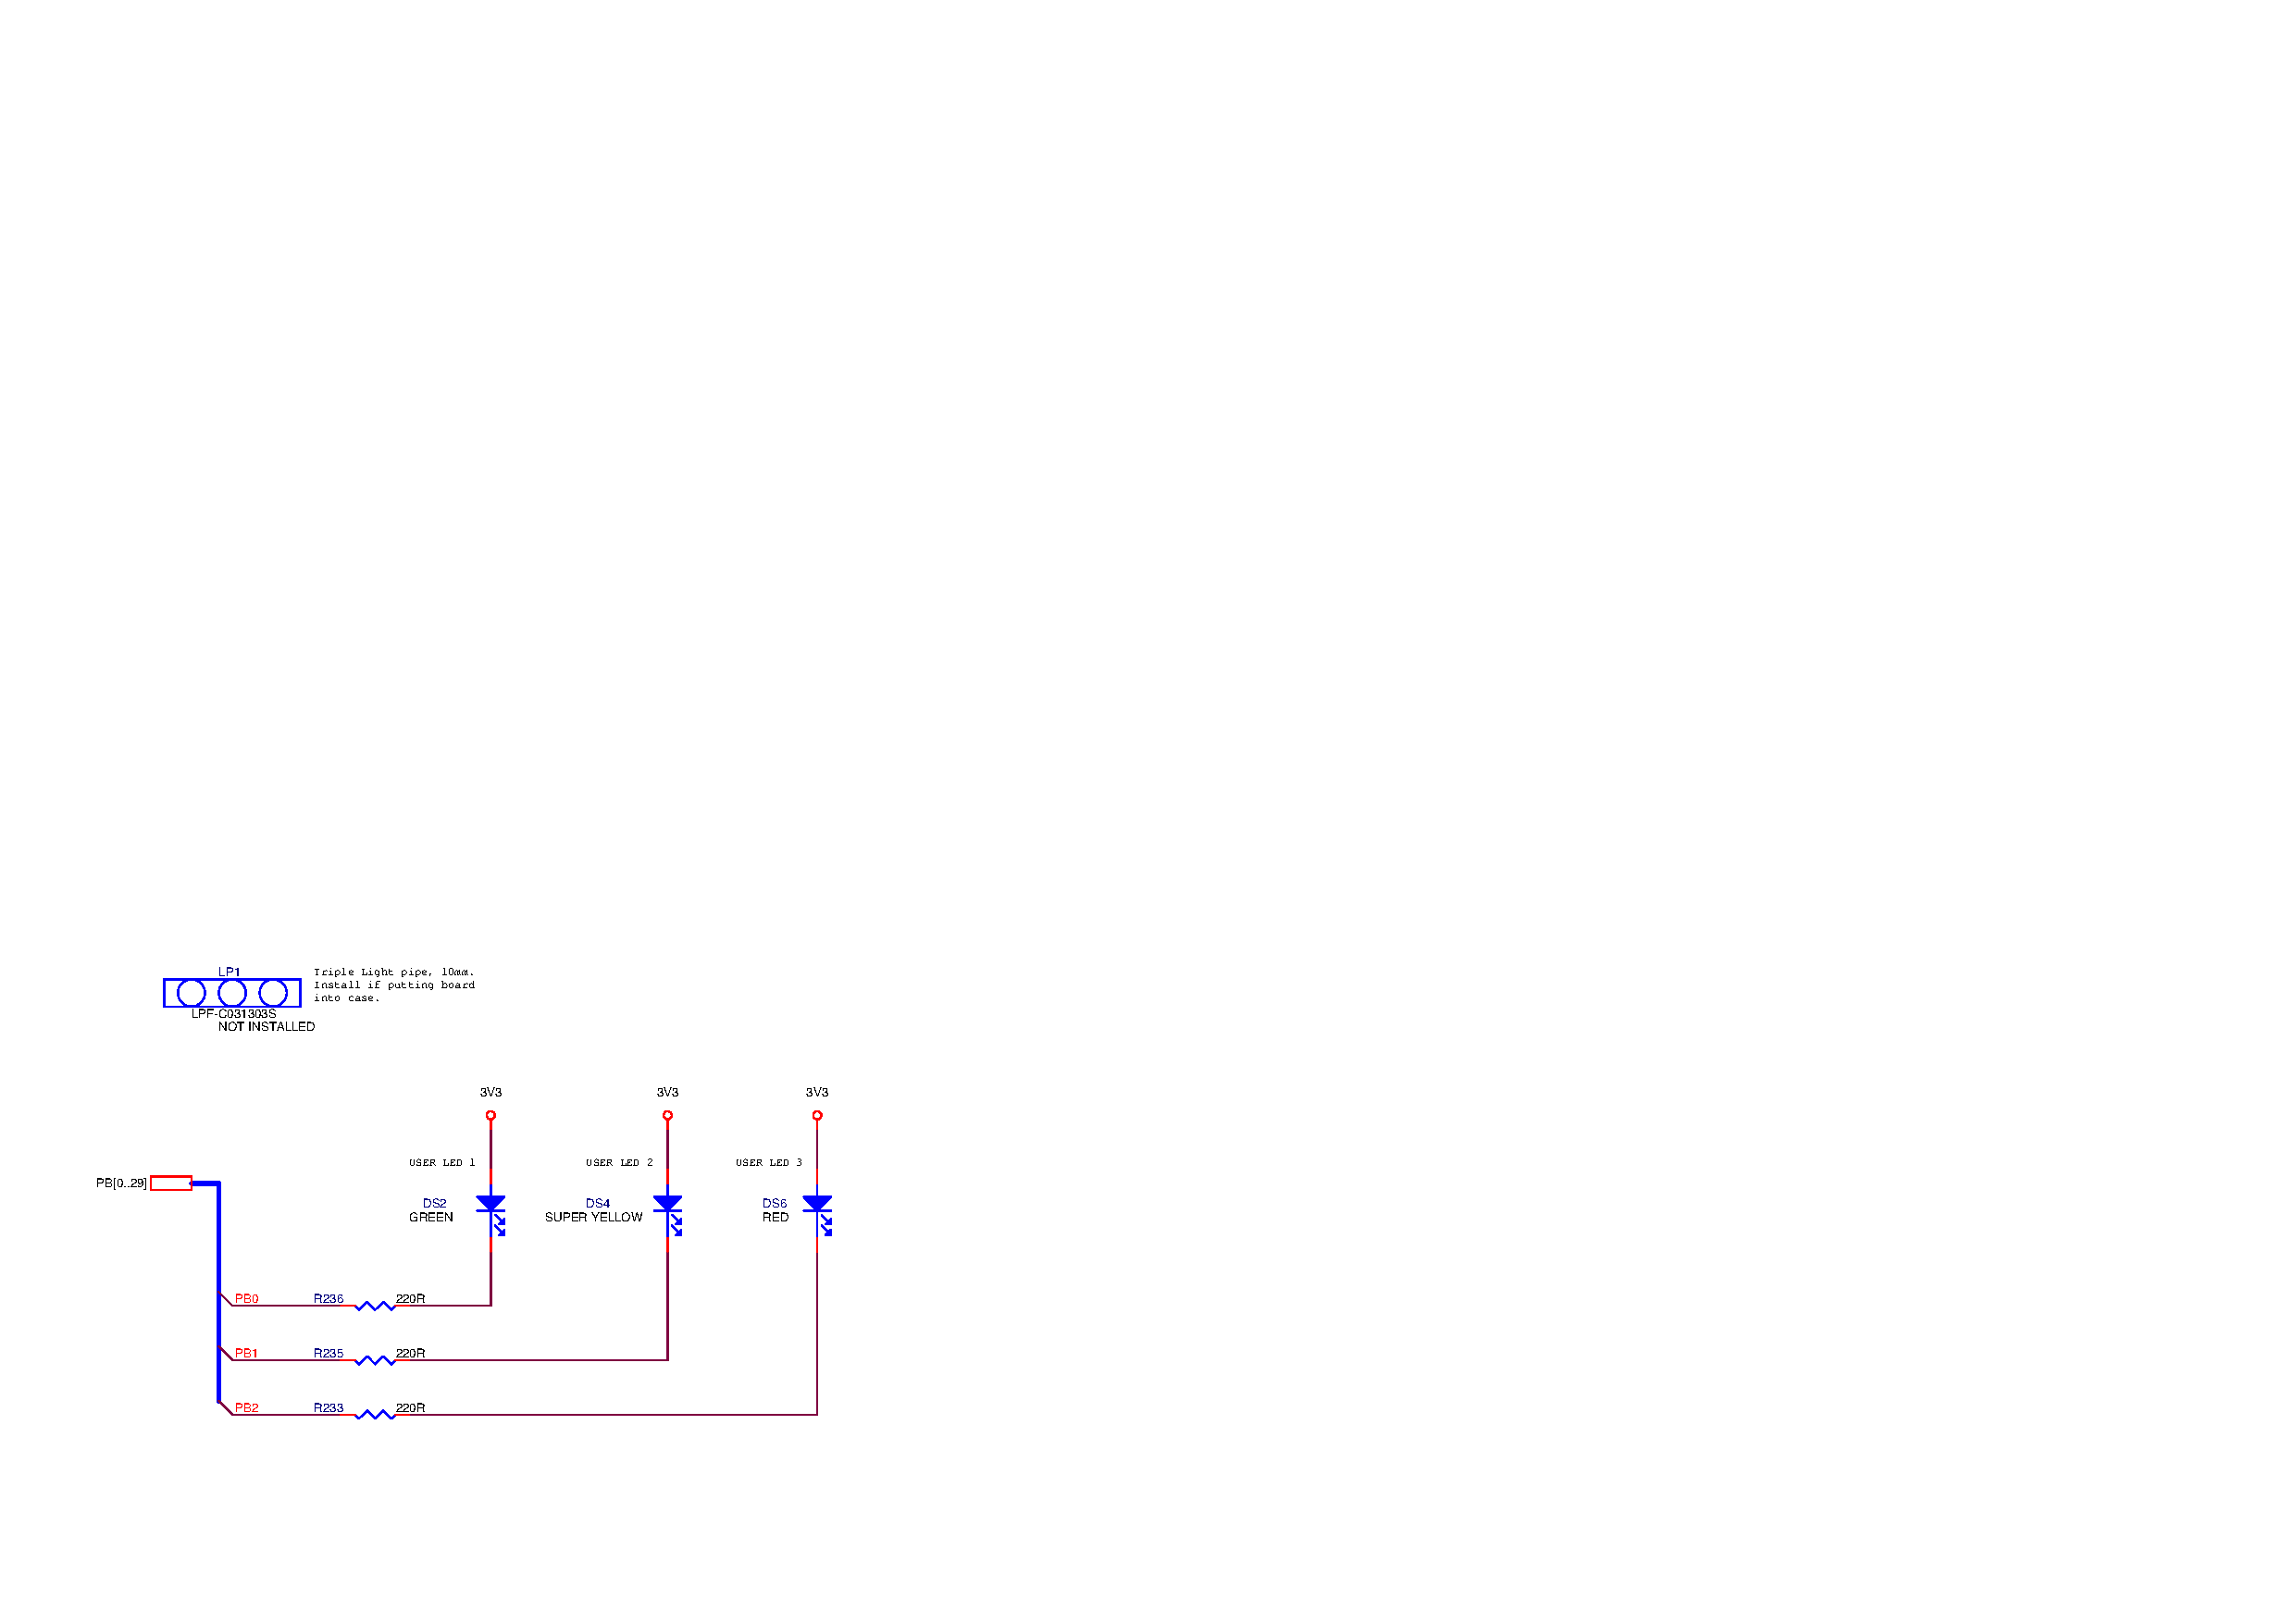
\includegraphics[width=0.8\textwidth]{images/LedScematic.pdf}
		\caption[LED Schematic AT91RM9200\_EK] {LED Schematic AT91RM9200\_EK \cite{AT91LED}}
	\label{fig:LEDsche}
\end{center}
\end{figure}




%\section{IO's}


\section{\acs{UART}}
\label{sec:RS232}
The \acf{UART} is a widely used interface in embedded systems. It's simple to configure and features flexible data rates as well as wiring length. Also different physical mediums can be used. The protocol transmit short messages containing only several bits. How ever there is is no clock synchronization, therefor the specified clock frequency has to have such a precision, to stay with in all bit timings of a transmitted frame. The interface features handshaking mechanism, but a simple serial bidirectional communication can be achieved with only 3 wires.\\
The used protocol in this project is the RS232. The features are transmission between 5 and maximally 9 bits of data. The frame itself begins with a start bit followed by the data. A one bit parity field allows error detection of all odd number of bit errors. The frame is ended 1,1.5 or 2 bits known as stop bit.\\
The RS232 specifies a negative logic for the computer to computer connection. The voltage levels need to be converted via a level converter into a positive logic with the processor voltage levels.\\
The \autoref{tab:RS232Set} shows the communication settings of the user as well as the debug interface. The handshaking mechanism is not used.\\

\begin{table}[H]
\begin{tabularx}{\textwidth}{llllll} %\hline
\textbf{Baud Rate}	 &\textbf{Data bits}  &\textbf{Parity} &\textbf{Stop Bit}&\textbf{Handshake}& \textbf{Type} \\
\hline
\hline
115200&8	& None & 1& Not used & Bidirectional\\
\end{tabularx}
\caption{User RS232 settings (8-N-1)}
\label{tab:RS232Set}
\end{table}

There are different methods for sending and receiving the data. The controller features a fully in hardware realized \ac{UART} transceiver. Therefor the received data is available for the application in a message buffer. For transmission a register used as a buffer to send out the data as soon as the there is no other data in transmission. The following enumeration explains 4 possible ways:

\begin{itemize}
	\item \textbf{Blocking:}\\
In case of receiving the application looks with a blocking function call if there is a new message in the buffer. If not it just loops the receiving status bit until there is new message available. This is called blocking, because the processor is fully occupied with the task of waiting till the status bit indicates successful received data.
For sending the core is blocked while waiting, before the data is stored in the transmission buffer. This is not suitable for an application, because if there is no data incoming or the transmission buffer is full, this will lead to a dead lock.\\
	\item \textbf{Polling:}\\
	An other possibility is the polling approach. This differs between the blocking in the way of testing if transmission or new data is present. The application can check time or event based and if the communication interface is not applicable, continue with its other tasks. The polling frequency needs to be higher as the baud rate of the \ac{UART}. How ever if the application load increases the the polling frequency (if not interrupt handled) decreases. This may lead to data loss on the receiving site or an decrease in data throughput on the sending side.\\
	\item \textbf{Interrupt:}\\
Interrupt handling for the receive case ensures no loss in data an a fast processing. As soon as valid data is available the generated interrupt executes the corresponding \ac{ISR}. The data is processed there. The core is only interrupted if new data is waiting for processing. In the case of no communication the processor has the full processing power to handle other tasks. To send data also an interrupt is generated when transmission is possible.
When there is long communication ongoing, the processors load is increased. The core has to serve the \ac{ISR} for every byte. This creates especially with high baud rates a high overhead for entering an exiting the \ac{ISR}.\\
	\item \textbf{\ac{DMA}:}\\
	To reduce the processor load, in the case of heavy communication, the \ac{DMA} controller is used. The feature of the memory access enables in the sending case to only specify a memory pointer and a data length. The peripheral \ac{DMA} controller then starts with the transmission till all data is transmitted. The processor therefor has to be interrupted only once. For receiving the \ac{DMA} can be configured in a way, such that all incomming data is stored into a specific location in the memory. An interrupt then could be triggered if the buffer is full or all data is available.\\
This method is used to transmit the result of the \ac{ILMS}. The AT91RM9200 features also a transmit next register to start a transmission right after the first one has finished.\cite{AT91DMA}\\
\end{itemize}


%################################################################################################

\newpage
%\subsection{USB}
\section{Digital Input}
For demo purpose (\autoref{DemoInt}) the duration of the high pulse of an digital input is measured. The distance measuring sensor unit (\autoref{UVsens}) is connected to the development board.\\
The microcontroller includes with the \acf{PIO} a fully programmable input/output controller. Other as in \autoref{sec:LED} the pin has to be configured as an input.\\
The controller provides features like, programmable pull up resistors, input glitch filter as well as an input change interrupt. Because of the connected input sensor neither input filtering nor a pull up resistor (connected on the sensor side) is necessary.\\ 
\autoref{IOCFG} gives an overview how the hardware input is configured. The InitDemoInterrupt function call (line 2) displays all function parameter by there mnemonic. At first the \ac{PMC} has to be configured (line 5). A special feature of the processor is \ac{PMC} peripheral clock configuration. The activation of the corresponding pin enables the update of the pin status with the master clock frequency. If not enabled the input pin stores the last level when a the clock was enabled. Best practice is to disable the input clock for not used inputs, after they have executed their last operation.\cite{AT91PMC}\\
To be able to read input signals the pin has to be configured as input. This is done with the AT91F\_PIO\_CfgInput-function. The function performs two operations. The output of this pin is deactivated and the pin is enabled.\\
Line 7 configures the \ac{AIC} (see \autoref{sec:AIC} for details) with the interrupt priority, the interrupt type and also the address where the \ac{ISR} is located. Line 8 and 10 enables the interrupt. First in the \ac{PIO}-controller and then in the \ac{AIC}.\\
Reading the \ac{PIO}\_ISR (Interrupt Status Register) is necessary because the hardware only features an change interrupt. So when ever the interrupt occurs before the programming of the \ac{AIC} or was not served the last time it needs to be cleared. This is done via reading the status register causing a clear of all pending \ac{PIO} interrupts. When then the next \ac{PIO} interrupts occurs the \ac{AIC} can serve the change and run the corresponding \ac{ISR}. An pending not served interrupt would be equivalent to a constant high level and would be never processed because of no change in the status register. Also any new interrupt would not affect this, because the status would just keep its value.\cite{AT91PIO}\\




\begin{lstlisting}[language=C, caption={Demo interrupt at PB15 configured as rising}, label={IOCFG}]
// Function call with parameters
	InitDemoInterrupt(AT91C_BASE_PIOB,AT91C_ID_PIOB, MY_INT_PIN, AT91C_AIC_PRIOR_LOWEST, AT91C_AIC_SRCTYPE_EXT_POSITIVE_EDGE);

void InitDemoInterrupt(AT91PS_PIO PIOptr, unsigned int ParallelID, unsigned int MyIOpin, unsigned int priority, unsigned int intType){
			AT91F_PMC_EnablePeriphClock (AT91C_BASE_PMC, ((unsigned int) 1 << ParallelID));
			AT91F_PIO_CfgInput (PIOptr, MyIOpin); 
			AT91F_AIC_ConfigureIt(AT91C_BASE_AIC,ParallelID,priority,intType,Measured_Interrupt_Lowlevel);
			AT91F_PIO_InterruptEnable (PIOptr, MyIOpin);
			{volatile unsigned int dummy; dummy = PIOptr -> PIO_ISR;}
			AT91F_AIC_EnableIt (AT91C_BASE_AIC, ParallelID); }
\end{lstlisting}

\subsection{Sharp sensor}
\label{UVsens}
The Sharp sensor GP2Y0D02YK0F (figure \ref{fig:sharpPic} is a distance measuring sensor with a range up to 80 cm. It provides an digital output high if an object is with in the range of the sensor. The measuring principle is based on an infrared emitting diode. Figure \ref{fig:sharpSchema} illustrates the different blocks of the sensor. The emitted light is processed in a position sensitive detector (PSD) and the signal processing circuit provides the digital output. To avoid toggling the sensor has a hysteresis of about 10 cm. Also because of the sensor design, measurements closer than approximately 4 cm are not possible. In conclusion with the in accuracy of the sensor the detecting range is between 4 cm and 80 $\pm$ 10 cm. The sensor needs a power supply of around 5V with maximally 50 mA of current. The output stage is a so called open collector output and needs an external pull up resistor around 12 k$\Omega$. The sensor is wired according to the recommended values. The power supply is connected to a \ac{USB} port of the development board. The output is connected to PB15 which is located at pin C42 of the expansion slot.\cite{sharp}\\

\begin{figure}[H]
\begin{center}
		  \subfigure[Sharp GP2Y0D02YK0F]{
    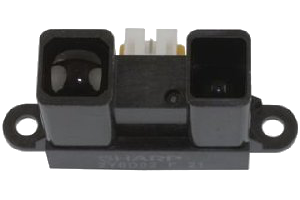
\includegraphics[width=0.42\textwidth]{images/GP2Y0D02YK0F.png}
		\label{fig:sharpPic}}
			\hspace{0.8 cm}
    \subfigure[Schematic of the sensor supply]{
   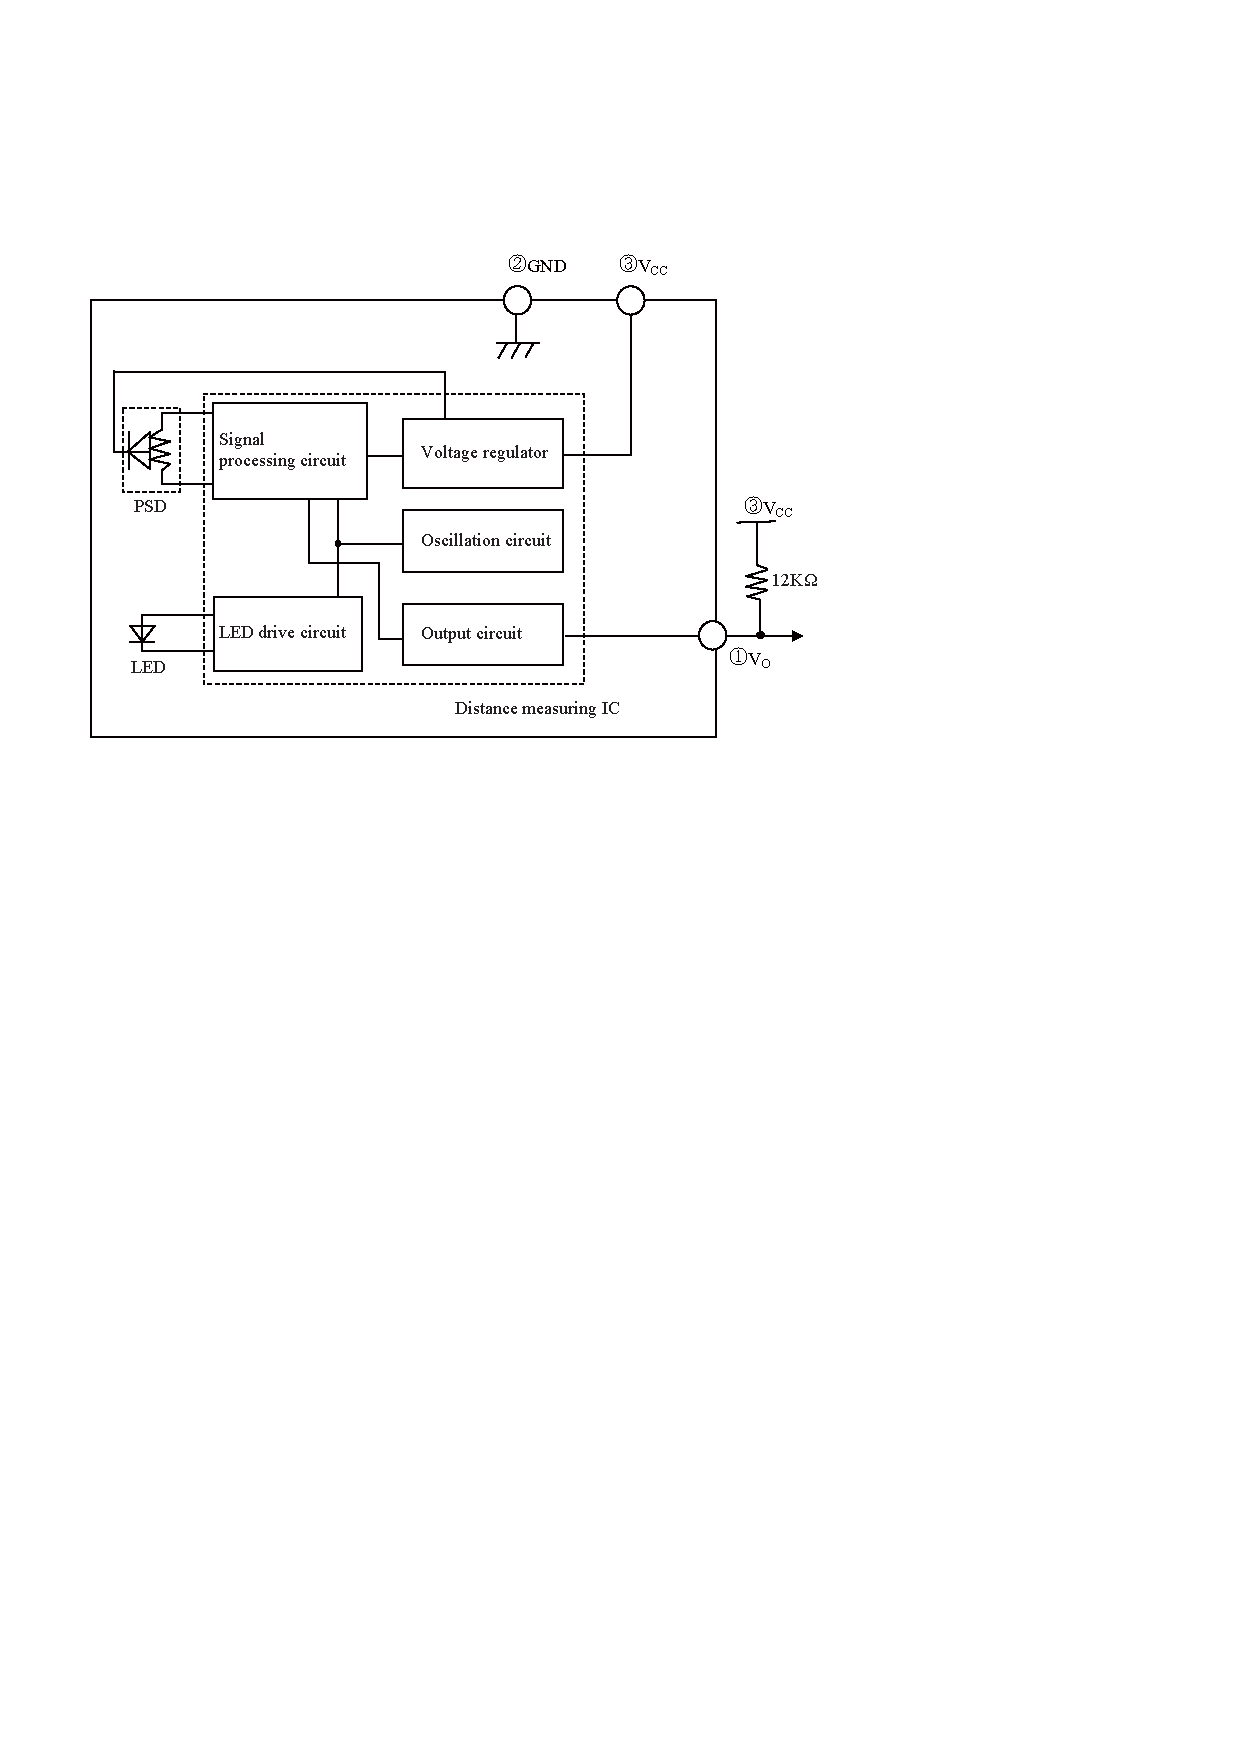
\includegraphics[width=0.42\textwidth]{images/SharpSchematics.pdf}
		\label{fig:sharpSchema}}
		\caption[Sharp GP2Y0D02YK0F Distance Measuring Sensor Unit]{Sharp GP2Y0D02YK0F Distance Measuring Sensor Unit \cite{sharp}}
		\label{fig:sharp}
		\end{center}
\end{figure}

\newpage
The sensor provides a stable output signal of around 40 ms. \autoref{fig:Sharptiming} displays the timing behavior of the sensor. The sensor update frequency is according to the timing limited by around 25 Hz. This is beneficial for the input of the microcontroller, because there is no need to filter this preprocessed, stable input signal. Line 4 in the \autoref{tab:Demointres} is a measurement of the shortest possible sensor high level duration. It is around 40.232 ms and with that in the range of the specified 38.3 $\pm$ 9.6 ms. Due to this fact all demo measurements of this table, are multiple of this duration. For example line 6 is a duration of 1167.025 ms and is approximately 29 times the minimum duration.\\

\begin{figure}[H]
\begin{center}
	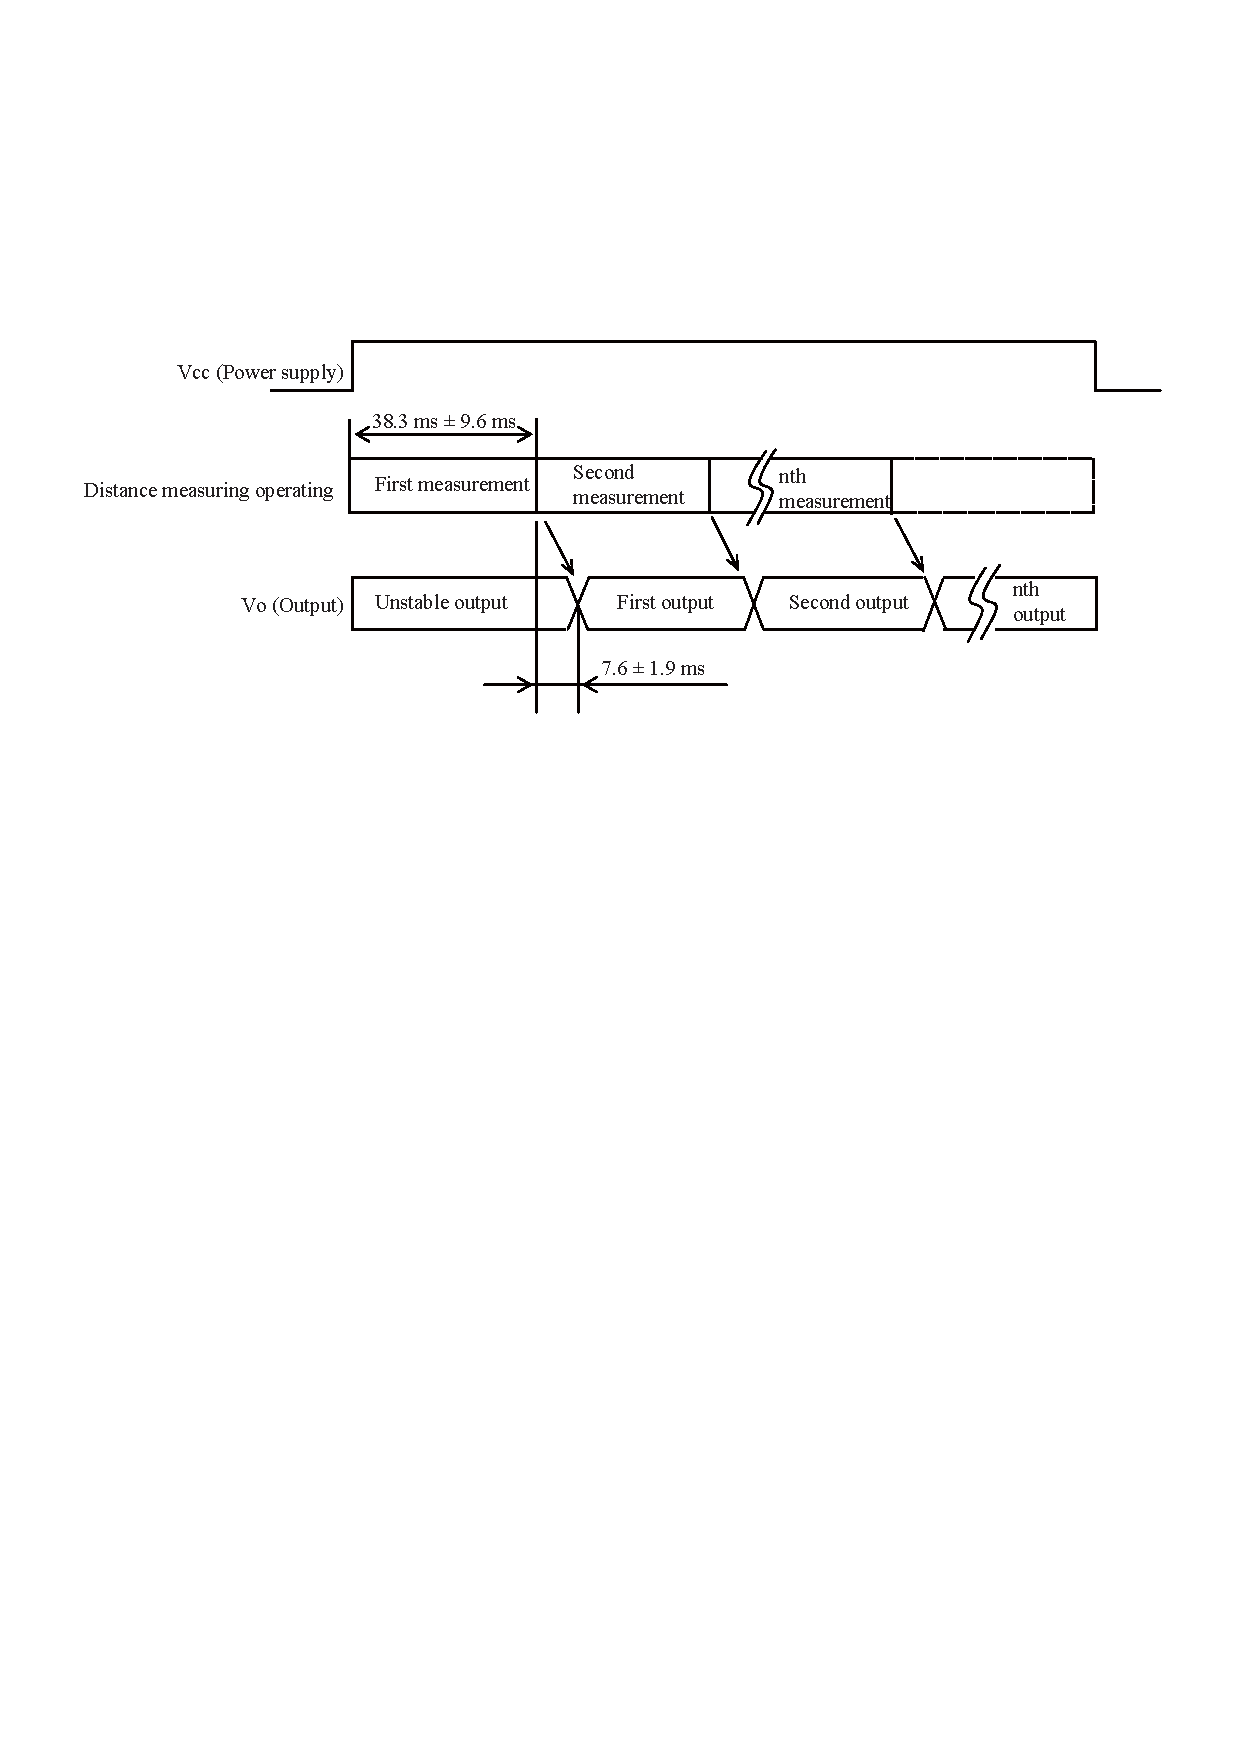
\includegraphics[width=0.8\textwidth]{images/SharpTiming.pdf}
		\caption[Sharp timing chart] {Sharp timing chart\cite{sharp}}
	\label{fig:Sharptiming}
\end{center}
\end{figure}



\section{\acs{RTC}}
\label{RTCchapter} 
The controller features a hardware \acf{RTC}. It's used inside this project to supply the date and time stamp when an measured interrupt has occurred. The \ac{RTC} has low power consumption and 200 year calendar. Also different interrupts can be triggered via programmable interrupts. The device uses the SLCK (32768 Hz) and divides this clock by 32768 to get a high precision 1 Hz clock. Time and date counting is done in hardware. The values are present in the \acf{BCD} format. This means each decimal is represented via 4 bits. Lower 4 bits encodes the unit and the upper 4 bits the tens.\cite{AT91RTC}\\
\autoref{RTCInit} lists the different commands to setup and initialize the \acs{RTC}. Line 3 checks and waits till the SEC flag is set. This is done because the user has to wait at least one second after the last update (only necessary for high frequent updating). Next the flags for updating time and date are set in the \acs{RTC} Control Register. The user also has to wait here, until the acknowledge is set in the \acs{RTC} Status Register. Line 6 selects the 24 hour mode. The next commands fills the date and time structures with the user defined settings. These two 32 bit values are stored in line 18 \& 19 in the \ac{RTC} time and date registers. These values are checked if they contain the right format and possible values. Otherwise the values are silently discarded. The clear in the next line disables the update request for time and date. The \ac{RTC} starts running again. And SEC flag is cleared with the next command to wait at least one second before re updating the time.\cite{AT91RTC}\\

\begin{lstlisting}[language=C, caption={Minimal \acs{RTC} initialization}, label={RTCInit}]
void Rtc_init(void) 
{	
	while (!(AT91C_BASE_RTC->RTC_SR & AT91C_RTC_SECEV) ); 
	AT91C_BASE_RTC->RTC_CR      = (AT91C_RTC_UPDTIM | AT91C_RTC_UPDCAL); 
	while (!(AT91C_BASE_RTC->RTC_SR & AT91C_RTC_ACKUPD) ); 
	AT91C_BASE_RTC->RTC_MR 		  = 0;         	
	rtc_time.time_bits.second 	= 0x00; 
	rtc_time.time_bits.minute 	= 0x35; 
	rtc_time.time_bits.hour 	  = 0x16; 
	rtc_time.time_bits.merid 	  = 0x00;
	
	rtc_cal.cal_bits.century 	  = 0x20; 
	rtc_cal.cal_bits.year 		  = 0x14; 
	rtc_cal.cal_bits.month 		  = 0x06; 
	rtc_cal.cal_bits.day 		    = 0x06; 
	rtc_cal.cal_bits.date 		  = 0x02;
	
	AT91C_BASE_RTC->RTC_TIMR    = (uint32)rtc_time.time_data;	
	AT91C_BASE_RTC->RTC_CALR    = (uint32)rtc_cal.cal_data;
	
	AT91C_BASE_RTC->RTC_CR 			= 0; 			
	AT91C_BASE_RTC->RTC_SCCR 		= AT91C_RTC_SECEV; 
}
\end{lstlisting}




%############################################################################################################

\chapter{Interrupt Latency Measurement Service}
\label{sec:ILMS}

The \acf{ILMS} provides a service to measure the computation time of interrupts. This could be used to check for real time capabilities of a measured task or record the worst case execution time in a test scenario. This is done by observing and recording any duration the interrupt needed with different load scenarios. Also long run times in terms of weeks or months may elongate interrupts and increase the used stack. This latency measurement is calculated with the \ac{ILMS} and transmitted over \ac{UART} (\autoref{tab:FC}) to a running and receiving database. A timestamp specifies the point in time when the execution of the interrupt started. For better readability this frame is transmitted as ASCII so also a standalone logging via a serial recorder is possible. The service is implemented in a way to use as less as possible resources of the processor and if possible compensate the measured result (see \ref{correction} for details). In order to archive for the application or programmer an easy way to specify a task to be measured, only the \ac{ISR} needs to be set to the "Measured\_Interrupt\_Lowlevel". The programmers \ac{ISR} then is automatically available as "Measured\_Interrupt\_Highlevel".\\
The main idea behind this is to start a timer, as soon as the low level routine is called through the \ac{AIC}. At this point also the time stamp is saved. After this the high level routine is loaded and executed. After the task is completed the timer is stopped and based on the timer and master clock frequency a duration of the task is calculated. The result is converted in to ASCII and transmitted via the \ac{DMA} through the \ac{UART} interface. This method allows an on chip measurement of the latency as well as serving nested interrupts.\\

\section{\ac{AIC}}
\label{sec:AIC}
The microcontroller includes also an \acf{AIC}. This allows the user to assign a priority form 0 to 7 for each interrupt source. That permits that higher prioritized interrupts to be executed even if a lower prioritized \ac{ISR} is executed at that time (interrupt nesting). The controller features different interrupt types for internal and external interrupts. Besides the priority, \acf{FIQ} and regular \acf{IRQ} can be processed. The \ac{FIQ} is always connected to the interrupt source 0. Banked registers enables a short context switch (\autoref{atcore} and \autoref{tab:regs}). Source 1 is reserved for system peripherals and source 2 to 31 for embedded peripheral or external interrupts. In this project the interrupt sources are, 3 for the digital input and 17 for the timer. The \ac{AIC} is not affected by the \ac{PMC} and no interrupt clock needs to be configured. Also vectoring provides an optimized way for branch and execution.\cite{AT91AIC}\\ % (\autoref{TimerCfg})

\section{\acs{ILMS} initialization}
The \ac{ILMS} provides 3 core functions. An extract of the "InterruptMeasurmentService.h" in \autoref{IMSH} displays these with their parameters. Before using the \ac{ILMS} the service needs to be initialized.\\
\begin{lstlisting}[language=C, caption={InterruptMeasurmentService.h functions}, label={IMSH}]
//InterruptMeasurmentService.h
void Init_Latency_Measurement	(unsigned char TimerClockBase,unsigned char TimerInterruptCompensation);
void Start_Latency_Measurement(void);
void Stop_Latency_Measurement	(void);
\end{lstlisting}
The init-command initialize the timer with the specified clock frequency. The mnemonics and resulting timer frequencies are specified in \autoref{tab:defines}. Also the last column indicates the maximum measurement duration without triggering an timer overflow (16 bit counter) at master clock speed of 60 MHz. Both input parameters are stored in the \ac{ILMS} environment to be used later on. Also a reconfiguration during run time would be possible. Similar to the I/O-configuration (\autoref{IOCFG}) the timer interrupt is configured and enabled. Compared to the lowest priority for the demo interrupt, the timer overflow requires the highest interrupt. This permits the overflow \ac{ISR} to be executed even if nested interrupts are being processed at this time (\autoref{timerovfl}.\\

\begin{table}[H]
\begin{tabular}{lllS[table-format=4.2]} %\hline
\textbf{Mnemonic}  &\textbf{Value} &\textbf{Description} &\textbf{Max. timer w/o ovfl @60MHz} \\
\hline
\hline
	 TIMER\_CLOCK1 		&0x00   &MCK/2  				& 2184.53 {$\;\mu s$}\\
	 TIMER\_CLOCK2 		&0x01		&MCK/8					&8738.13 {$\;\mu s$}\\
	 TIMER\_CLOCK3 		&0x02		&MCK/32					&34.95 {$\;m s$}\\
	 TIMER\_CLOCK4 		&0x03		&MCK/128				&139.81{$\;m s$}\\
	 TIMER\_CLOCK5 		&0x04		&SLCK (32768Hz)	&2.00 {$\;s\;$}\\
	\hline
	 INT\_COMP\_OFF 		&0x00		&\multicolumn{2}{l}{Correction disabled}\\
	 INT\_COMP\_ON 		&0x01	  &\multicolumn{2}{l}{Correction enabled}\\
\end{tabular}
\caption{mnemonic for timer and interrupt compensation}
\label{tab:defines}
\end{table}
The second function parameter describes if the time compensation for the timer overflow interrupted should be activated or is not required. Subsection \ref{correction} describes the used time approximation. The following enumeration gives examples when to use the compensation and also application where there is no need or a compensation would sophisticate the result:\\
\begin{itemize}
	\item \textbf{INT\_COMP\_OFF:}\\
	Should be used for all sorts of hardware inputs. In general where there are two separate events when the task is started and ended. E.g. input pulse width measurement. Like in the demo interrupt the measurement is started with the rising edge and ended by the falling edge of the digital I/O.\\
	
	\item \textbf{INT\_COMP\_ON:}\\
	For all measured long tasks which fully use the full processor power from start to finish. They could be interrupted by higher prioritized interrupts. How ever a scheduled task can be measured, but depending on the processor load the task may is not elongated through the timer overflow \ac{ISR} and the compensation should be turned off.
\end{itemize}
In general there is no difference for short tasks whether the compensation is active or not. This is only true as long as there is no timer overflow. The clock frequency of the timer (\autoref{tab:defines}) therefor should be a compromise between accuracy and the maximum measurable time span. To just pick the SLCK as the slowest frequency would enable measurements up to 2 s without an timer overflow. However the accuracy per tick is with 30.52 $\mu s$ (master clock 60 MHz) rather low.\\


\section{Interrupt concept}
As mentioned in \autoref{sec:ILMS}, the \ac{ILMS} provides the low level routine with a fixed callback to the application / programmer specified high level \ac{ISR}. \autoref{MILSR} is an extract of the "ISR.S". This part provides low level function. The interrupt entry macro in line 10 switches the processor mode and pushes the user register in the user stack. Also the link register is updated.\\
The "bl" command starts the interrupt latency measurement. The mnemonic branch with link adjust the \ac{PC} to the specified address and updates the link register to continue after the start with the "ldr" command (line 15). The start of the measurement clears the timer overflow counter, starts the timer and saves the time stamp.\\
The lines 15-17 are the equivalent to the bl command. However they display each step of loading the to branch address, adjusting the return address and updating the \ac{PC}. \\




\begin{lstlisting}[language=Assembler, caption={Measured interrupt low level service routing}, label={MILSR}]
@------------------------------------------------------------------------------
@ Measured_Interrupt_Lowlevel
@------------------------------------------------------------------------------
	.global Measured_Interrupt_Lowlevel
	.extern Measured_Interrupt_Highlevel
  .extern Start_Latency_Measurement
	.extern Stop_Latency_Measurement
	
Measured_Interrupt_Lowlevel:
	IRQ_ENTRY

	@Branch with Link to start the the interrupt latency measurement
	bl			Start_Latency_Measurement  

	ldr     r1, =Measured_Interrupt_Highlevel
	mov     r14, pc
	bx      r1
	
	@Branch with Link to Stop the interrupt latency measurement
	bl 			Stop_Latency_Measurement
		
	IRQ_EXIT
@------------------------------------------------------------
\end{lstlisting}
The after the high level routine was executed the "Stop\_Latency\_Measurement" is processed. At first the timer is stopped and the the overflow interrupt is disabled. A get time function combines the current 16 bit timer status together with the overflow to an 32 bit timer value. The unit here is ticks and needs to be converted with the knowledge of the timer frequency into $\mu s$. This is done with the "Convert\_Ticks\_To\_us"-function (\autoref{c2us}). The number of ticks was recorded in case "TIMER\_CLOCK2" with 1/8 MCK. With one arithmetic logical shift left (multiplication with the factor 2) and the devise by 15 a resulting division of 7.5 is realized. The timer clock frequency oscillates with 7.5 MHz therefore 7.5 ticks are equivalent to one $\mu s$. This is also done for the other clocks. The return value of the function is the measured time in microseconds.\\ 

\begin{lstlisting}[language=Assembler, caption={Extract Convert\_Ticks\_To\_us-function}, label={c2us}]
unsigned int Convert_Ticks_To_us (unsigned int Ticks,unsigned char TimerClockBase)
{ 
	 switch (TimerClockBase)
	 {
	 case TIMER_CLOCK1:
			return Ticks/30; 				//Tested [v]
		
	 case TIMER_CLOCK2:
			return (Ticks<<1)/15; 	//Tested [v]
	 //. . .
\end{lstlisting}

\subsection{Time correction}
\label{correction}
%Together with the timer clock frequency and the stored number of timer overflows, the total ticks can be computed. The value is then based on the clock frequency converted in an integer containing the time in $\mu s$.
Then depending on the state of the state of the stored variable, the compensated time is calculated by subtracting a correction factor.\\ 

\begin{table}[H]
\begin{tabular}{llll} %\hline
\textbf{Scope}	&\textbf{Part} &\textbf{Assembly lines}  &\textbf{Processor cycles} \\
\hline
\hline
Lowlevel:\\
\cline{1-1}
				& IRQ\_Entry 	&		8& 13\\
				&Other				&	3&3\\
				& IRQ\_Exit 	&7&12\\
Highlevel:\\
\cline{1-1}
				& Acknowleg int 	&		8& 8\\
				& resetLED(RED)				&	3&3\\
				& TimerOverflowCnt++ 	&3&3\\ \hhline{~~~=} 

&&&	42 (approx.)\\			
\end{tabular}
\caption{Additional processors cycles per timer overflow}
\label{tab:addCycles}
\end{table}

The correction tries to calculate the time spend to load, process and exit the timer {ISR}, elongating the measured interrupt. To calculate this the assembly code for the interrupt entry and exit macros (\autoref{IRQEntry} and \autoref{IRQExit}) together with the timer overflow assembly code is used. Most of the assembly instructions are single cycle operations. \autoref{tab:addCycles} estimates the required clock cycles. The timer \ac{ISR} it self contains no branches so no pipeline drop is expected. The start and stop of the timer are almost atomic instructions and only needed once and are therefor neglected. Due to simplicity and with a master clock of 60 MHz the correction assumes 60 clock cycles for a full service of the timer overflow interrupt. This leads that if the compensation is enabled for every overflow 1 $\mu s$ is subtracted from the measurement result.\\

\noindent\begin{minipage}{.45\textwidth}
\begin{lstlisting}[language=Assembler,caption={IRQ\_Entry},label={IRQEntry}]
@- IRQ Entry
@-----------
.macro	IRQ_ENTRY
sub     lr, lr, #4
stmfd   sp!, {lr}
ldr     r14, =AT91C_BASE_AIC
str     r14, [r14, #AIC_IVR]
mrs     r14, SPSR
stmfd   sp!, {r14}
msr     CPSR_c, #ARM_MODE_SYS 
stmfd   sp!, { r0-r3, r12, r14}
.endm
\end{lstlisting}
\end{minipage}\hfill
\begin{minipage}{.45\textwidth}
\begin{lstlisting}[language=Assembler,caption={IRQ\_EXIT},label={IRQExit}]
@- IRQ Exit
@-----------
.macro  IRQ_EXIT
ldmia   sp!, { r0-r3, r12, r14}
msr     CPSR_c, #I_BIT | 
				ARM_MODE_IRQ
ldr     r14, =AT91C_BASE_AIC
str     r14, [r14, #AIC_EOICR]
ldmia   sp!, {r14}
msr     SPSR_cxsf, r14
ldmia   sp!, {pc}^
.endm
\end{lstlisting}
\end{minipage}

\subsection{Timestamp and result conversion}
The stored date and time has to be converted into ASCII characters. Due to the fact that all values are stored as \ac{BCD} the conversion can be made rather simple  compared to the result value. The index inside the costant arry Dec2ASCII (\autoref{D2ASCII}) is used to select the correct corresponding ASCII value of each number. This is done for the unit and tens separately by masking and shifting.\\
\begin{lstlisting}[language=C,caption={Constant Dec2ASCII},label={D2ASCII}]
const unsigned char Dec2ASCII[]="0123456789";
\end{lstlisting}
This could be also done by just adding the offset between number and ASCII value (decimal 48). Each value is then stored in the correct place inside the date and time string. The whole conversion is repeated until time and date stamp is completed. The time and date separator between the digits could be chosen individual to enhance readability.\\ 
The measured interrupt latency is stored in an unsigned integer (32 bit) and has to be converted into ASCII as well to be transmitted via the serial connection. The function "Dec2ASCII\_Ticks" (\autoref{Res2ASCII}) also takes care of storing the converted values into the "ASCII\_UART\_Buffer". The constant MEASVALOFF is the offset between the position of the time stamp and the result inside the buffer. The core concept of the function is to convert the value into ASCII and if the value is smaller as the maximum number of characters to fill this blank with the blank symbol (second function parameter). To achieve the conversion the unsigned integer value is divided via the Divider variable. The result of the integer division is then compared if it's greater than zero. And if so the value is converted via the addition of decimal 48 and stored into the buffer. Also the indication number has occurred ("numberoccurred") is set to true. If the value is zero the blank symbol is filled into the buffer. The remaining integer number is calculated via the modulo operator. Also the Divider is down scaled by the factor 10. In the second round of the for loop the integer division is calculated. The if statement does a disjunction with the now may set "numberoccoured". This is necessary that now the zero value instead of the blank symbol should be used if there was a previous other digit than zero.\\
The whole for loop is run exactly 10 times and therefor has a almost constant conversion time independence from the value that needs to be converted. The blank symbol helps to achieve a constant length to ensure the frame format and readability. A demo recording result  is shown in \autoref{tab:Demointres}.\\

 
\begin{lstlisting}[language=C,caption={Result to ASCII conversion},label={Res2ASCII}]
void Dec2ASCII_Ticks(unsigned int value,unsigned char blanksym)
{	unsigned char numberoccoured=0;
	unsigned int num;
	unsigned int ValToWork=value;
	unsigned int i;
	unsigned int Divider=1000000000;
	
	for(i=0;i<10;i++)
	{	
		num=ValToWork/Divider;
			if(num|numberoccoured)
			{			ASCII_UART_Buffer[i+MEASVALOFF]=(unsigned char)num+48;
						numberoccoured=1;															}
			else
			{			ASCII_UART_Buffer[i+MEASVALOFF]=blanksym; 		}
		ValToWork\%=Divider;
		Divider/=10;
	}
}
\end{lstlisting}








\subsection{Measurement transmission}
The complete string is after the update of time stamp and measurement result ready to be transmitted. This is done via the \ac{DMA}. The transmission routine there selects the user RS232 and sets the message address as well as the number of bytes to be transmitted. The routine needs this information to program the \ac{DMA} register. Depending on the current transmission state, either the transmit pointer register or if a transmission is on going the transmit next pointer register is set\footnote{If no register is available, the transmission is dropped. The function returns with an error code (not handled)}.\\
The full string is then transmitted. \autoref{TransTime} calculates the transmission time for one full message: 
\begin{align}
String\_length \times Bits\_per\_character \div	Bits\_per\_second\;&=\;  Transmission\_time\notag\\ 
34 \times 10 \div 115200\;&=\;2.86\;ms
\label{TransTime}
\end{align}

Each of the 34 characters (\autoref{tab:FC}) is transmitted with one start and one stop bit. This results in the number "bits per character". With the baud rate of 115200 bits per second one message needs less than 3 ms to be sent. 
With the whole process of converting the time and date to ASCII as well as the value transmission, the \ac{ILMS} is limited by around 4 ms. Therefor sporadic interrupts could be handled once via the "`next transmission \ac{DMA} register. But the whole \ac{ILMS} is not able to serve higher interrupt frequencies than approximately 25 Hz without improvements (see \autoref{improv} for suggestions).



\subsubsection{RS232 frame format}
\autoref{tab:FC} specifies the transmitted string with all sections to be received and processed with the database or stand alone software. The Datestamp contains only numbers and has a part length\footnote{Including space character at the end (see \autoref{tab:Demointres} for details)\label{inklSpace}} of 11 characters. The Timestamp contains 9 characters\footref{inklSpace} followed by the result with a length\footref{inklSpace} of 11. The string is completed by the unit $\mu s$ and the "\textbackslash n" with 3 characters.\\   

\begin{table}[H]
\begin{tabular}{llllll} %\hline
\textbf{Frame}	 &\textbf{Datestamp} &\textbf{Timestamp} 		&\textbf{Measurement} 	&\textbf{Unit} &\textbf{Delimiter} \\
\hline
\hline
Symbolic				&DD/MM/YYYY			&HH:MM:SS									& Value						& Unit  & \textbackslash n \\ %\cline{1-2}
Example				&18/05/2014			&15:57:30								& 0000123456						& $\mu s$  & \textbackslash n \\ %\cline{1-2}

\end{tabular}
\caption{RS232 Frame Components}
\label{tab:FC}
\end{table}






%\subsubsection{Interrupt configuration}

%\subsubsection{Timer configuration}
%\label{TimerCfg}

\newpage
\subsection{Measurement scenarios}
\label{timerovfl}
There are various scenarios of interrupt occurrence possible. \autoref{fig:IntEX} gives an overview about 3 different measured interrupts. In general the time axis of the figures features no time unit and is only used to reference for the event description. The time between two timestamps doesn't have to be of the same duration. The left column descries different tasks. The application has in this example no priority\footnote{Priorities are referenced by the \ac{AIC} priority}. A rising arrow from one task indicates an interruption of the this task. An arrow in downwards direction indicates the \ac{ISR} of the higher priority task was completed and the interrupted task continue to run. In terms of the \ac{ILMS} there is no additional interrupt after starting the measurement and the measured interrupt. This is a normal (callback) function call and is indicated with a line with no arrowhead. The whole chart is organized from top down starting with the highest priority.\\
In figure \ref{fig:IntExa} a short interrupt is measured. The application is in running state until at time point 2 an interrupt for the measured interrupt occurs. The \ac{ILMS} starts its service by saving the \ac{RTC} values and starting the timer. With a normal function call the \ac{ISR}, which has to be measured, is loaded. The measured \ac{ISR} then is active in the example till moment 5. The \ac{ILMS} then stops the Timer and triggers the the time calculation and correction as well as the conversion to ASCII. The service sets the \ac{DMA} for the auto transmission of the result string and returns to continue the main application. The message then is transmitted in parallel while the application already is executed. Because of the time constraint due to a transmission time of around 4 ms the \ac{ILMS} is not able to measure interrupts which occur and finish in less than 4 ms in a short time range.\\
For a visual explanation it is assumed that timer stop and the conversion of the measurement result takes around 1 ms (time between point 5 and 6). The application becomes running again and the transmission of the 34 byte string takes according to \autoref{TransTime} less then 3 ms. So the complete string would be transmitted until point 9 on the scale. This would allow a new result transmission. With the \ac{DMA} next transmission buffer this would be possible once\footnote{\ac{ILMS} used only one message buffer} in a short time period, until both buffers are available again. Therefor especially high frequent, low computing time interrupts are not measurable.\\
In the figure \ref{fig:IntExa} the interrupt occurs at point in time 10 so every 8 instant of time and is handled and measured in the same way as the interrupt at time 2.\\
In figure \ref{fig:IntExab} a long \ac{ISR} has to be measured. Like in the previous example the application is running and is interrupted at time point 2 to execute a measured interrupt. After the start of timer and the store of the start time the measured interrupt is executed. It is active until point in time 5.5. At this moment an timer overflow occurs. The timer is configured with a high priority permitting the timer \ac{ISR} to interrupt the measured interrupt. The timer overflow then is active till point 6 of the scale. While being active the interrupt is acknowledged and an counter, counting the number of overflows, is increased. As well as for demo purpose the "RED" LED is turned off. The falling arrow indicates that the prior \ac{ISR} was served. The metered interrupt then becomes active and continues until time point 8. This example indicates an clock frequency of the timer which leads to an overflow every 2.5 time units with a timer overflow computation time of 0.5 units. This influences especially for high clock frequency an elongation of the measured interrupt. However this is necessary due to the fact that the timer registers are 16 bit. The interrupt continues and is one more time interrupted by the timer overflow until it stops the measurement at point 10. Like in the previous example the time is calculated and converted into $\mu s$. Now it depends on the timer configuration if the time in the timer overflow \ac{ISR} is subtracted from the result (see \autoref{correction}). The result then is send via the RS232 while the application continues.\\
Figure \ref{fig:IntExac} is an example of an long measured interrupt with timer overflows and other higher prioritized interrupts intercepting the \ac{ISR} of the measured interrupt. Also in this example the application is running and interrupted at point 2. The \ac{ILMS} starts the measurement and continues with the metered interrupt. This one is active (ACT) until point in time 4. The Example contains multiple system interrupts (System Int a,b,c). These interrupts could be also other user or peripheral interrupts with higher priorities compared to the measured interrupt. After the intercept System Int c) is active. This one is also interrupted by the timer overflow interrupt having the highest priority in the whole scenario. This one is like previous configured to occur every 2.5 time units. After the timer \ac{ISR} has been executed the System Int c) continues for 0.5 time slice and is interrupted by the higher prioritized System Int b). At time point 7.5 then the highest System Int a) occurs and is served. After the timer interrupt at time 8 the whole chain then follows in descending order the measured interrupt then is executed again. Between time 10 and 15 two more timer interrupts and one System Int b) is processed. The time is then stopped and converted and send to the stand alone or database server software. In this example the measured interrupt would only need 3.5 time units to be completed. But this execution time is not reached due to the higher priorities competing for processor time. Instead in this case the interrupt has an execution time of 12 units without compensation. In case of normal operation there would be then no timer interrupt and the execution time would be 10 units.\\ 
In longtime measurements the execution time of different scenarios could be measured and recorded to figure out the worst case execution time of one task. The results then can be checked against possible critical deadlines for this specific task\\
%-----------------------
\begin{figure}[H]
		\begin{center}
		% Time skale vektor
\newcommand{\timingaxis}[1][]{%
  \begin{scope}[#1]
  \draw [timing/table/axis] (0,-\nrows) -- (\twidth+1,-\nrows);
	\draw (\twidth+1,-\nrows-0.1)node [below,inner sep=2pt] {\scalebox{.75}{\tiny t}};
  \foreach \n in {0,1,...,\twidth} {
    \draw [timing/table/axis ticks]
        (\n,-\nrows+.1) -- +(0,-0.2)
        node [below,inner sep=2pt] {\scalebox{.75}{\tiny\n}};
  }
  \end{scope}
}
\tikzset{%
    timing/table/axis/.style={->,>=latex},
    timing/table/axis ticks/.style={},
}
% ---------------------  
		
		
		
		
		
		
		\subfigure[Short measured interrupt, no timer overflow or competing other interrupts]{
			\begin{tikztimingtable}[
							timing/slope=0,         % no slope
							timing/coldist=2pt,     % column distance
							%timing/rowdist=0.34cm,
							timing/coldist=0.25cm,
							timing/rowdist=0.75em,
							timing/yunit=0.75em,
							xscale=2,yscale=1.0, % scale diagrams
							timing/d/background/.style={fill=white},
							thick               % set line width
						]
						{Timer overflow}     						& [orange]    										\\
						{}															& [black]																	\\%Arrow
						{System Int a)}     						& [black] 										\\
						{}															& [black] 									\\%Arrow
						{System Int b)}     						& [black] 										\\
						{}															& [black] 										\\%Arrow
						{System Int c)}     						& [black] 										\\
						{}															& [black] 															\\%Arrow
						{Measured Interrupt} 						& [red]  3S0U2D{Active}0U 6S 2D{Active}0U  \\
						{}															& [black]3S 0G 2S 0G 6S 0G 2S 0G						\\%Arrow
						{\acs{ILMS}} 										& [blue]  2S0U1D{Start}0U2S0U1D{Stop}0U4S0U1D{Start}0U2S0U1D{Stop}0U       		        \\
						{}															& [black]2S 4A 4W 4A W																						\\%Arrow
						{Application} 								  & [green]  0U2D{ Running }0U4S0U4D{ Running }0U4S0U4D{Running}0U              \\
					\extracode
					\makeatletter
					\timingaxis%\relax
					 \begin{pgfonlayer}{background}
						% Draw shaded backgrounds
						\shade [right color=orange!20,left color=orange!20](0,1.0) rectangle (\twidth+2.5,0.0);
						\shade [right color=yellow!20,left color=yellow!20] (0,-1.0) rectangle (\twidth+2.5,-6.0);
						\shade [right color=red!20,left color=blue!20] (0,-7.0) rectangle (\twidth+2.5,-10.0);
						\shade [right color=green!20,left color=green!20](0,-11) rectangle (\twidth+2.5,-12);
					 
						% Add background grid lines
						\begin{scope}[gray,semitransparent,semithick]
							\horlines{1,3,...,13}
							\foreach \x in {0,...,18}
								\draw (\x,1) -- (\x,-\nrows);
							% similar: \vertlines{1,...,6}
						\end{scope}
						% Add labels
						\node [anchor=west,inner sep=0pt] at (\twidth+0.1,0.5) {\tiny Prio: High};
						\node [anchor=west,inner sep=0pt] at (\twidth+0.1,-1.5) {\tiny Prio: Mid 3};						
						\node [anchor=west,inner sep=0pt] at (\twidth+0.1,-3.5) {\tiny Prio: Mid 2};
						\node [anchor=west,inner sep=0pt] at (\twidth+0.1,-5.5) {\tiny Prio: Mid 1};
						\node [anchor=west,inner sep=0pt] at (\twidth+0.1,-7.5) {\tiny Prio: Low};
						\node [anchor=west,inner sep=0pt] at (\twidth+0.1,-11.5) {\tiny Prio: None};
					 \end{pgfonlayer}
					\end{tikztimingtable}%

		\label{fig:IntExa}}\\
		\vspace{0.5 cm}
    \subfigure[Long measured interrupt, with timer overflow but no competing other interrupts]{
    						 \begin{tikztimingtable}[
							timing/slope=0,         % no slope
							timing/coldist=2pt,     % column distance
							%timing/rowdist=0.34cm,
							timing/coldist=0.25cm,
							timing/rowdist=0.75em,
							timing/yunit=0.75em,
							xscale=2,yscale=1.0, % scale diagrams
							timing/d/background/.style={fill=white},
							thick               % set line width
						]


						{Timer overflow}     						& [orange] 5.5S0U0.5D 0U2S0U0.5D0U    										\\
						{}															& [black] 5.5S 0.5A 0G 2S 0.5A 0G 													\\%Arrow
						{System Int a)}     						& [black] 5.5S 0G	0.5S 0G 2S 0G 0.5S 0G 										\\
						{}															& [black] 5.5S 0G	0.5S 0G 2S 0G 0.5S 0G										\\%Arrow
						{System Int b)}     						& [black] 5.5S 0G	0.5S 0G 2S 0G 0.5S 0G									\\
						{}															& [black] 5.5S 0G	0.5S 0G 2S 0G 0.5S 0G 										\\%Arrow
						{System Int c)}     						& [black] 5.5S 0G	0.5S 0G 2S 0G 0.5S 0G										\\
						{}															& [black] 5.5S 0G	0.5S 2W 0G 0.5S W																\\%Arrow
						{Measured Interrupt} 						& [red]  3S0U2.5D{Active}0U0.5S0U2D{Active}0U0.5S0U1.5D{Active}0U   \\
						{}															& [black]3S 0G 7S 0G 																						\\%Arrow
						{\acs{ILMS}} 										& [blue]  2S0U1D{Start}0U7S0U1D{Stop}0U       		        \\
						{}															& [black]2S 9A W 																						\\%Arrow
						{Application} 								  & [green]  0U2D{ Running }0U9S0U7D{ Running }0U              \\
					\extracode
					\makeatletter
					\timingaxis%\relax
					 \begin{pgfonlayer}{background}
						% Draw shaded backgrounds
						\shade [right color=orange!20,left color=orange!20](0,1.0) rectangle (\twidth+2.5,0.0);
						\shade [right color=yellow!20,left color=yellow!20] (0,-1.0) rectangle (\twidth+2.5,-6.0);
						\shade [right color=red!20,left color=blue!20] (0,-7.0) rectangle (\twidth+2.5,-10.0);
						\shade [right color=green!20,left color=green!20](0,-11) rectangle (\twidth+2.5,-12);
					 
						% Add background grid lines
						\begin{scope}[gray,semitransparent,semithick]
							\horlines{1,3,...,13}
							\foreach \x in {0,...,18}
								\draw (\x,1) -- (\x,-\nrows);
							% similar: \vertlines{1,...,6}
						\end{scope}
						% Add labels
						\node [anchor=west,inner sep=0pt] at (\twidth+0.1,0.5) {\tiny Prio: High};
						\node [anchor=west,inner sep=0pt] at (\twidth+0.1,-1.5) {\tiny Prio: Mid 3};						
						\node [anchor=west,inner sep=0pt] at (\twidth+0.1,-3.5) {\tiny Prio: Mid 2};
						\node [anchor=west,inner sep=0pt] at (\twidth+0.1,-5.5) {\tiny Prio: Mid 1};
						\node [anchor=west,inner sep=0pt] at (\twidth+0.1,-7.5) {\tiny Prio: Low};
						\node [anchor=west,inner sep=0pt] at (\twidth+0.1,-11.5) {\tiny Prio: None};
					 \end{pgfonlayer}
					\end{tikztimingtable}%
		\label{fig:IntExab}}\\
		\vspace{0.5 cm}
		\subfigure[Long measured interrupt, with timer overflow and other higher prioritized interrupts]{
    						\begin{tikztimingtable}[
							timing/slope=0,         % no slope
							timing/coldist=2pt,     % column distance
							%timing/rowdist=0.34cm,
							timing/coldist=0.25cm,
							timing/rowdist=0.75em,
							timing/yunit=0.75em,
							xscale=2,yscale=1.0, % scale diagrams
							timing/d/background/.style={fill=white},
							thick               % set line width
						]


						{Timer overflow}     						& [orange] 5.5S 0U0.5D0U2S 0U0.5D0U2S 0U0.5D0U2S 0U0.5D0U2S   \\
						{}															& [black] 5.5S0A0.5S0G2S0A0.5S0W2S0A0.5S0G2S0A0.5S0G2S	\\%Arrow
						{System Int a)}     						& [black] 5.5S0G0.5S0G1.5S 0U[brown]0.5D0U0.5S0U0.5D0U [black]1.5S0G0.5S0G2S0G0.5S0G\\
						{}															& [black] 5.5S0G0.5S0G1.5S0A1.5S0W1.5S0G0.5S0G2S0G0.5SW								\\%Arrow
						{System Int b)}     						& [black] 5.5S0G0.5S0G0.5S 0U[cyan]1D{Int B}1.5S0.5D0U [black]1S0G0.5S0G 1S 0U[cyan]1D0U0.5S0U0.5D0U			\\
						{}															& [black] 5.5S0G0.5S0.5W 3A 1W 0G 0.5S 0G 1S 2A G						\\%Arrow
						{System Int c)}     						& [magenta] 4S0U1.5D{Int C} 0.5S0U0.5D0U 3S0U0.5D0U	[black]0.5S0G0.5S0G1S0G2S0G \\
						{}															& [black] 4S6A0W0.5S0G0.5S1W0G2SW															\\%Arrow
						{Measured Interrupt} 						& [red]  3S0U1D{ACT}0U 6S0U0.5D0U 0.5S0U1D0U 2S0U1D0U  \\
						{}															& [black]3S 0G 12S 0G 																				\\%Arrow
						{\acs{ILMS}} 										& [blue]  2S0U1D{Start}0U12S0U1D{Stop}0U       		        \\
						{}															& [black]2S 14A W 																						\\%Arrow
						{Application} 								  & [green]  0U2D{ Running }0U14S0U2D{ Running }0U              \\
					\extracode
					\makeatletter
					\timingaxis%\relax
					 \begin{pgfonlayer}{background}
						% Draw shaded backgrounds
						\shade [right color=orange!20,left color=orange!20](0,1.0) rectangle (\twidth+2.5,0.0);
						\shade [right color=yellow!20,left color=yellow!20] (0,-1.0) rectangle (\twidth+2.5,-6.0);
						\shade [right color=red!20,left color=blue!20] (0,-7.0) rectangle (\twidth+2.5,-10.0);
						\shade [right color=green!20,left color=green!20](0,-11) rectangle (\twidth+2.5,-12);
					 
						% Add background grid lines
						\begin{scope}[gray,semitransparent,semithick]
							\horlines{1,3,...,13}
							\foreach \x in {0,...,18}
								\draw (\x,1) -- (\x,-\nrows);
							% similar: \vertlines{1,...,6}
						\end{scope}
						% Add labels
						\node [anchor=west,inner sep=0pt] at (\twidth+0.1,0.5) {\tiny Prio: High};
						\node [anchor=west,inner sep=0pt] at (\twidth+0.1,-1.5) {\tiny Prio: Mid 3};						
						\node [anchor=west,inner sep=0pt] at (\twidth+0.1,-3.5) {\tiny Prio: Mid 2};
						\node [anchor=west,inner sep=0pt] at (\twidth+0.1,-5.5) {\tiny Prio: Mid 1};
						\node [anchor=west,inner sep=0pt] at (\twidth+0.1,-7.5) {\tiny Prio: Low};
						\node [anchor=west,inner sep=0pt] at (\twidth+0.1,-11.5) {\tiny Prio: None};
					 \end{pgfonlayer}
					\end{tikztimingtable}%
					\label{fig:IntExac}}\\
		\vspace{0.5 cm}
		\caption{Example of possible interrupts occurrence and the corresponding handling}
		\label{fig:IntEX}
		\end{center}
\end{figure}
%--------------------------


\newpage
\subsection{Demo interrupt function}
\label{DemoInt}
The demo interrupt uses the output signal of the sharp distance sensor (\autoref{UVsens}) to trigger an interrupt when an obstacle is in range of the sensor. The high level routine is executed after the start of the \ac{ILMS}. \autoref{DemoIntISR} gives an overview of the main part of the high level \ac{ISR}. For demo purpose and as an user feed the GREEN LED is turned on. With the while loop (line 5) the controller stays in that interrupt as long as the obstacle is not removed in front of the sensor. This serves as measurement of the high period of the sensor. After the while loop is break the LED is turned off\footnote{Toggling of the YELLOW LED is done every time after the \ac{ILMS} is stopped} and the high level is completed. During this the \ac{ILMS} clocked the execution (in this case high duration time). After completion the value is then converted an send to the Database or stand alone software.\\
In the case of a duration measurement the compensation for the timer overflow interrupt should be turned of. How ever this waiting for low could be also seen as demonstration what could happen if other task interrupt the removing of the obstacle. In terms of the processor this means what happens if there are other higher priorities interrupting and elongating the measured interrupt like in figure \ref{fig:IntExac}.

\begin{lstlisting}[language=C,caption={Extract of the demo interrupt high level \ac{ISR}},label={DemoIntISR}]
void  Measured_Interrupt_Highlevel (void)
{			// . . .
	
			setLed(GREEN);
			while(AT91F_PIO_GetInput (AT91C_BASE_PIOB) & MY_INT_PIN); // Wait if high!
			resetLed(GREEN);

			// . . .					}
\end{lstlisting}
\autoref{tab:Demointres} is an extract of an record of interrupt measurements created with the demo interrupt and the sharp distance sensor.
\begin{table}[H]
\begin{tabular}{l}  %\hline
\textbf{Measurement Result} \\
\hline
\hline
18/05/2014\textvisiblespace 16:59:39\textvisiblespace 0000080460\textvisiblespace us\textbackslash n\\
18/05/2014\textvisiblespace 16:59:41\textvisiblespace 0000080456\textvisiblespace us\textbackslash n\\
18/05/2014\textvisiblespace 16:59:43\textvisiblespace 0011866587\textvisiblespace us\textbackslash n\\
18/05/2014\textvisiblespace 17:00:07\textvisiblespace 0000040232\textvisiblespace us\textbackslash n\\
%18/05/2014\textvisiblespace 17:29:09\textvisiblespace 0002776273\textvisiblespace us\textvisiblespace \textbackslash n\\
%18/05/2014\textvisiblespace 17:29:12\textvisiblespace 0000563274\textvisiblespace us\textvisiblespace \textbackslash n\\
%18/05/2014\textvisiblespace 18:28:52\textvisiblespace 0000120712\textvisiblespace us\textvisiblespace \textbackslash n\\
%18/05/2014\textvisiblespace 18:28:54\textvisiblespace 0000120708\textvisiblespace us\textvisiblespace \textbackslash n\\
%18/05/2014\textvisiblespace 18:28:55\textvisiblespace 0000965858\textvisiblespace us\textvisiblespace \textbackslash n\\
%18/05/2014\textvisiblespace 18:28:56\textvisiblespace 0000845122\textvisiblespace us\textvisiblespace \textbackslash n\\
%18/05/2014\textvisiblespace 18:28:57\textvisiblespace 0000442668\textvisiblespace us\textvisiblespace \textbackslash n\\
18/05/2014\textvisiblespace 18:28:58\textvisiblespace 0000120731\textvisiblespace us\textbackslash n\\
18/05/2014\textvisiblespace 18:28:59\textvisiblespace 0001167025\textvisiblespace us\textbackslash n\\
%18/05/2014\textvisiblespace 18:34:07\textvisiblespace 0000080490\textvisiblespace us\textvisiblespace \textbackslash n\\
%18/05/2014\textvisiblespace 18:34:09\textvisiblespace 0002736411\textvisiblespace us\textvisiblespace \textbackslash n\\
%18/05/2014\textvisiblespace 18:34:14\textvisiblespace 0005754692\textvisiblespace us\textvisiblespace \textbackslash n\\
%18/05/2014\textvisiblespace 18:34:23\textvisiblespace 0010181320\textvisiblespace us\textvisiblespace \textbackslash n\\

\end{tabular}
\caption{Demo interrupt results}
\label{tab:Demointres}
\end{table}

\chapter{Conclusion}
The \ac{ILMS} enables a precise time measurement of the interrupt execution time. By using the internal timer there is no need for external hardware or a co-processor. The time spent in the timer overflow can be estimated and corrected. By using the highest priority for the timer overflow, also nested interrupts can be served. It is then also possible to measure the execution time of a \ac{FIQ}-\ac{ISR} if no timer overflow occurs\footnote{The time between an interrupt becoming pending until the start of execution (including the context switch) is not measured with the \ac{ILMS} and would require a major change in the interrupt concept}. The timer frequency is configurable and should be set as a trade of between accuracy or time without an timer overflow. In general a precision of $1\;\mu s$ and a maximum duration of around 5 s can be achieved. The \ac{RTC} provides the start time and date stamp when an interrupt occurred. Together with the value the whole measurement is transmitted as a 34 byte string. The frame format then can be processed in a database software. An ASCII character format ensures also readability via a serial monitor but also limits the \ac{ILMS} in terms of the ability to measure high frequent interrupts. A demo interrupt was used to check the measured results for plausibility.\\

\section{Further improvements}
\label{improv}
\begin{itemize}
	%\item \textbf{Flexible message with or without timestamps}\\
	
	\item \textbf{Flexible configuration}\\
				The \ac{ILMS} could be configured via RS232 by the user or the database software.
				\begin{itemize}
						\item Messages with or without time and/or date stamp.
						\item Timer frequency selection.
						\item Accuracy selection (selection of the base time unit or a flexible configuration e.g. 3 fractional digits).
						\item Enable or disable the time correction.
						\item Configuring whether the \ac{RTC} is saved at interrupt occurrence or completion.
						\item RAW mode for database high speed transmission. (4 byte UNXI timestamp, 4 byte result and fixed unit ticks).
						\item Flexible date and time transmission (only included if there was a change in the values), 					requires reliable message transmission.
				\end{itemize}
	
	\item \textbf{Message buffering}\\
				 Message buffering and reliable transmission with message acknowledge / handshaking mechanism. Scalable message buffer.
	
	\item \textbf{Resynchronizing of the RTC}\\
				The \ac{RTC} time could be synchronized via DCF77 receiver. Through an DCF77 decoder time and date is coded via a pulse width modulation. After a frame is successfully received the time could be updated every minute. This would require one more system timer. 
	\item \textbf{Result plausibility  check}\\
				Use a second timer with a slow frequency to compute the measured time to. This would allow to the detect if e.g. when metering the \ac{FIQ} timer overflow were missed. Also if the results would differ if 32 aren't enough to store the value.
	
	%\item \textbf{Flexible timestamps before the interrupt or after it finishes}\\
	
	\item \textbf{Timer selection and priority}\\
	Flexible configuration of the used timer and warning when application uses the same timer. Also e.g. macro based checking if the timer functionality can be achieved (has the timer a higher priority than the measured interrupt or is the timer in use).
	
\end{itemize}

